% As of May 2025, this DocumentMetadata is required for creating a tagged pdf
% which supports alt text for images and other accessibility features.
% See https://latex3.github.io/tagging-project/ for the latest information
% on creating accessible tagged pdfs with LaTeX.

% If part of your thesis or dissertation is not working with tagging
% you will get errors with "Package tagpdf Error" you can disable tagging
% for part of your document by using 
%  \tagpdfparaOff 
%  [... code that is causing problems ...]
%  \tagpdfparaOn

\DocumentMetadata{
	lang=en,
	testphase={phase-II,graphic}
}
\documentclass[thesis]{MSUstyle}
%
%  Created by Seth Humphries 
%  Update and maintained by Prof. Mark Owkes mark.owkes@montana.edu
% 
%%    Copyright (c) 2007-2012 Seth D. Humphries
%%    This work is licensed under the Creative Commons
%%    Attribution-Noncommercial-Share Alike 3.0 License. To view a copy
%%    of this license, visit http://creativecommons.org/licenses/by-nc-sa/3.0/;
%%    or, (b) send a letter to Creative Commons, 171 2nd Street, Suite
%%    300, San Francisco, California, 94105, USA. 
%
%  Version 2.0, check for periodic updates on the bitbucket repository
%
% DEFAULTS --------------------
% The default options are as follows:
%   \documentclass[12pt,letterpaper,oneside,openright,%
%       doublespaced,normalmargins,dissertation,final,numreset]{MSUstyle}
%
% default options do not need to be entered. Defaults will generate a document 
% that conforms to the MSU Electronic Thesis/Dissertation  (ETD) guidelines. 
%
% MASTERS THESIS ---------------
%  use \documentclass[thesis]{MSUstyle} to adjustment the front matter according to ETD style rules that
% are different for a thesis than for a dissertation.
%
% ADDITIONAL OPTIONS ----------
% 10pt, singlespaced, and draft allow you to require less number of pages for editing
% A draft version number can be set with, e.g., \draftver{1.0}
%
% numberedsections provides numbered chapter and section titles
%
% appendsingle/appendmultiple is required if you have one/multiple appendices, remove if you do not have an appendix
%
% nonumreset does not add chapter to labels of figures, tables, etc. (not recommended)
%
% PRINTING OPTIONS ------------
% oneside,openright (defaults) 1" margin on all sides of pages (use for electronic documents and submission to grad school)
% oneside,openright,bigmargin larger margin on left side of pages (optionally use for electronic documents and submission to grad school)
% twoside,openright  1" margins,  blank pages added so chapter start on right page (use for printing on minimal number of pages)
% twoside,openright,bigmargin larger margins alternate left/right sides for binding and ...
%                               blank pages added so chapter start on right page (use for nicest printed material)

% ========================= %
%  Packages                 %
%  (add as needed)          %
% ========================= %
\usepackage[final]{graphicx} %for the \includegraphics command and figures put [final] before ...
%%    {graphix} if you want figures to show up even while in draft mode
\usepackage{subcaption}    % to be able to have multiple plots in one figure
\usepackage{color} % for changing text color in chapters \textcolor{red}{red text read here}. 
\usepackage{varioref}  % for \vref{figure} which shows up like ``figure 4 on page 6'' 
\usepackage[final]{listings} % used for formatting code
\usepackage[numbers,sort&compress]{natbib} % for citations
\usepackage{longtable} % for long nomenclature (and other long tables)

\usepackage{tikz} % used for creating figures
\usetikzlibrary{calc}
\usetikzlibrary{patterns}
\usetikzlibrary{positioning}
\usetikzlibrary{decorations.markings}
\usetikzlibrary{decorations.pathmorphing}
\usetikzlibrary{arrows}

\usepackage{amsmath}
\usepackage{lipsum} % Generates random text
%\usepackage{showframe} % View margins

\usepackage{booktabs}
\usepackage{siunitx}

% Style of code listings (Change as needed)
\lstset{%set Code listings styles
	language=Matlab, % program language for keywords and comments styles
	basicstyle=\small, %font size and style
	identifierstyle=\color{red}, %variable name style
	stringstyle=\ttfamily, %string style
	keywordstyle=\color{blue}\bfseries, %language keyword style
	commentstyle=\color{black}\itshape, %commentstyle
	breaklines=true,  % sets automatic line breaking
	breakatwhitespace=false,   %break line not just at whitespaces
}


% ======================= %
%  User defined commands  %
% ======================= %
\newcommand{\etc}{etc.}
\newcommand{\eg}{e.g.}
\newcommand{\ie}{i.e.} 
\DeclareSIUnit{\rpm}{rpm}
\DeclareSIUnit{\inch}{in}
\DeclareSIUnit{\ampererms}{A_{rms}}
%REVIEW-ADD-BEGIN
% ==================================================================== REVIEW
% REVIEW MARKUP (added for Draft 1 review, Nov. 2026). Nothing in the
% chapter files was removed: suggested deletions are struck through and
% kept in the source.
%   \add{...}   blue           suggested new text
%   \del{...}   red, struck    suggested deletion (\cancel inside math)
%   \note{...}  orange         reviewer comment, never part of the thesis
%   delblock    red block      suggested deletion of whole paragraphs,
%                              equations, or tables
% \showeditstrue  : show all markup (review copy)
% \showeditsfalse : accept every suggestion (adds kept, deletions and
%                   notes hidden)
% Remove this block, and the markup, once all edits are resolved.
\usepackage[normalem]{ulem}
\usepackage{cancel}
\usepackage{comment}
\definecolor{revadd}{rgb}{0,0,0.85}
\definecolor{revdel}{rgb}{0.8,0,0}
\definecolor{revnote}{rgb}{0.85,0.42,0}
\newif\ifshowedits
\showeditstrue
% siunitx macros cannot be split by \sout; box them inside \del.
\AtBeginDocument{%
  \NewCommandCopy{\RevOrigSI}{\SI}\NewCommandCopy{\RevOrigsi}{\si}%
  \NewCommandCopy{\RevOrignum}{\num}\NewCommandCopy{\RevOrigqty}{\qty}%
  \NewCommandCopy{\RevOrigang}{\ang}}
\NewDocumentCommand{\RevSIbox}{O{}mom}{\mbox{\IfValueTF{#3}%
  {\RevOrigSI[#1]{#2}[#3]{#4}}{\RevOrigSI[#1]{#2}{#4}}}}
\NewDocumentCommand{\Revsibox}{O{}m}{\mbox{\RevOrigsi[#1]{#2}}}
\NewDocumentCommand{\Revnumbox}{O{}m}{\mbox{\RevOrignum[#1]{#2}}}
\NewDocumentCommand{\Revqtybox}{O{}mm}{\mbox{\RevOrigqty[#1]{#2}{#3}}}
\NewDocumentCommand{\Revangbox}{O{}m}{\mbox{\RevOrigang[#1]{#2}}}
\ifshowedits
  \newcommand{\add}[1]{{\color{revadd}#1}}
  \newcommand{\del}[1]{\ifmmode{\color{revdel}\cancel{#1}}\else
    {\color{revdel}\let\SI\RevSIbox\let\si\Revsibox\let\num\Revnumbox%
     \let\qty\Revqtybox\let\ang\Revangbox\sout{#1}}\fi}
  \newcommand{\note}[1]{{\color{revnote}[\textbf{Note:} #1]}}
  \newenvironment{delblock}%
    {\par\color{revdel}\noindent\textbf{[Suggested deletion: start]}\par}%
    {\par\noindent\textbf{[Suggested deletion: end]}\par}
\else
  \newcommand{\add}[1]{#1}
  \newcommand{\del}[1]{}
  \newcommand{\note}[1]{}
  \excludecomment{delblock}
\fi
% ================================================================ END REVIEW
%REVIEW-ADD-END
%REVIEW-ADD-BEGIN
% ============================================================ FIGURES
% \thesisfigure[width]{name}{alt text}
% Looks for figures/name.pdf, .png, or .jpg. If the file exists it is
% included with its alt text (used by the tagged PDF). Until then a
% framed placeholder with the file name and alt text is drawn, so the
% thesis compiles before the figures exist. Put finished figures in a
% folder named "figures" next to main.tex using the names given.
\newcommand{\thesisfigure}[3][0.9\linewidth]{%
  \IfFileExists{figures/#2.pdf}{\includegraphics[width=#1,alt={#3}]{figures/#2.pdf}}{%
  \IfFileExists{figures/#2.png}{\includegraphics[width=#1,alt={#3}]{figures/#2.png}}{%
  \IfFileExists{figures/#2.jpg}{\includegraphics[width=#1,alt={#3}]{figures/#2.jpg}}{%
  \fbox{\parbox[c][0.22\textheight][c]{\dimexpr#1-2\fboxsep-2\fboxrule\relax}{%
    \centering\small\textbf{Figure placeholder:}
    \texttt{figures/\detokenize{#2}}\\[1ex]
    \parbox{0.9\linewidth}{\raggedright\footnotesize\textit{Alt text:} #3}}}}}}}
% ======================================================== END FIGURES
%REVIEW-ADD-END
% =============================== %
%  Definitions: Change as needed  %
% =============================== %
\name{Chris Jordan Doe} %PUT your FULL name here (First Middle Last)
\DocTitle{This is the title of your thesis or dissertation \\ which may span multiple lines \\ (but no more than 3 lines) } 
\OWNwebpage{http://mywebsite.net} %your personal webpage
\degreetitle{Engineering} % may be different than department... ie MS in Electrical Engineering is not Elect. and Com. Engnr degree.
\department{Electrical and Computer Engineering} 
\committeechair{Dr. Kevin S. Repasky} 
\departmentchair{Dr. Robert C. Maher}
\graduatedean{Dr. Carl A. Fox}
\graduationdate{May 2025}
\copyrightyear{2025} % add one to year if document submitted in Dec.
%\draftver{1.0} % versioning for use with draft option

% put searchable words you want internet search engines to find here
\keys{Engineering, PhD, Dissertation, Template, Latex, Montana, Montana State University} 
 
%  Configuration of hyperref package
\hypersetup{%
	baseurl={\OWNwebpage}, %baseurl is url that is in pdf document properties
% 	bookmarks=true, %show bookmarks when opening pdf
	citecolor=black, %citations show up black
	colorlinks=true, %use colored links
   %draft=false, % prevents hyperref from draft mode...keeps bookmarks and hyperlinks in draft mode
	filecolor=black, %included file links are black text
	linkcolor=black, %the colored links are black for an ETD but can be otherwise
	pdfauthor={\name}, %pdf document maker is you
	pdfcreator={\name \ by \ PDFLaTex}, %pdf document maker is you
	pdfdisplaydoctitle=true, % make display title the same as the document title instead of the filename
	pdffitwindow=true, %fits one page into the open pdf reader window
	pdfkeywords={\keys}, %searchable keywords
	pdfsubject={\degreetype \ for \name}, %the \  is to give a space
	pdftitle={\DocTitle}, %pdf document title is now ETD title
	plainpages=false, %use hyperlinks in pages, gets rid of a lot of warnings too
	urlcolor=black %website links are black text
}%

% ================================ %
%         Actual Document                                              %
% ================================ %
\begin{document}

% Front matter...before your text
\begin{preliminary} 

  % Dedication page (optional, comment out if not using)
  \begin{dedication} 
    % Dedication

I dedicate this to all MSU students who use \LaTeX.  Dedication is optional and may be no longer than one page, single spaced, and should precede the acknowledgments page.  


 
  \end{dedication}

  % Acknowledgements page (optional, comment out if not using)
  \begin{acknowledgements}
    % Acknowledgement

I would like acknowledge\dots Acknowledgments must be double spaced and is limited to one page. Consider that you may need to include a funding acknowledgement.

 
  \end{acknowledgements}

  %vita page (optional, comment out if not using)
  \begin{vita}
    % Vita

Chris Jordan Doe was born in Bozeman, MT in 1893.  Raised by Champ, Chris is a true Bobcat. Chris attended Bozeman High and graduated with honors. After high school, \dots

If you include a vita, it should contain the full name of the author, date and place of birth, parentage, secondary education, and collegiate degrees. The vita should be written in essay form in the third person and may not exceed one single-spaced page.

 
  \end{vita}

  % Table of Contents, List of Figures|Tables|etc.
  \contents

  % Nomenclature page (optional, comment out if not using)
  \begin{nomen}
    % Nomenclature 
\setlength\LTleft\parindent
\setlength\LTright\fill
\begin{longtable}{l l}
  $\mu$ & Dynamic viscosity \\
  $\mathbf{n}$ & Normal vector\\
  $\mathbf{u}$ & Velocity vector
\end{longtable}

% Reset table counter to back to zero so the first actual table is labeled table 1
\setcounter{table}{0} 
  \end{nomen}

  % Abstract
  \begin{abstract}
    % Abstract 
The abstract must be single spaced and no more than 350 words. The abstract must contain the following elements: (1) statement of the problem, (2) procedure or methods, (3) results, and (4) conclusions. Mathematical formulas, abbreviations, diagrams, and other illustrative materials should not be included. It should be written to be understood by a person who does not have expertise in the field.

  \end{abstract}
\end{preliminary}

% Dissertation chapters:  add/change as needed
\chapter{Introduction}\label{CH:introduction}
 Modern manufacturing relies heavily on producing precise, intricate metal components. This is often achieved through subtractive manufacturing techniques using equipment such as milling machines and lathes. These machines have been in use for approximately two hundred years \cite{groover_fundamentals_2010,moriwaki_multi-functional_2008}, and during this time have been continually improved. Manual control of these machines has been incrementally replaced by increasingly capable computerization \cite{reintjes_numerical_1991,groover_fundamentals_2010}. Modern milling machines and lathes often use Computer Numerical Control (CNC), which removes the need for a human machinist to control each detail of the machining process through manual inputs \cite{groover_fundamentals_2010}. Due to this continued computerization, these machines have grown in complexity, enabling more advanced machining operations, including advanced work with ductile materials, brittle materials, and increasingly complex part geometry \cite{moriwaki_multi-functional_2008,sheng_review_2026}. Continued development has also introduced new systems to these machines, including systems that allow the Machine to autonomously detect in real time a broken tool and replace the tool, detect abnormally high stress loads, or monitor motor loads across the machine. These innovations are significant because they enable the machines to autonomously catch in real time errors that previously would have been caught by a human, and with CNC machines could have propagated into damaged parts or damaged machines. These innovations work to reduce scrap part rates, damaged tooling, and critically machine downtime \cite{nagaraj_tool_2025,wong_technical_2020}.


\section{Machining Overview}\label{machiningOverview}
\subsection{Lathe}\label{Sect:lathe}
A lathe performs subtractive manufacturing by rotating the workpiece around the spindle axis, designated as the Z axis, while translating the cutting tool in the X and Z axes. The X axis is commonly used to move the tool radially and controls the finished diameter of the workpiece. The Z axis moves along the length of the workpiece and is used to control the axial extent of the cut. Given the workpiece rotates while the tool traverses a plane containing the axis of rotation, all features are produced as surfaces of revolution that are axially symmetric about the Z axis \cite{altintas_manufacturing_2012}. Lathes are commonly used to achieve part geometries that require turning outer diameters, boring internal diameters, facing, and drilling and tapping holes along the Z axis. Contoured profiles, including hemispherical and other curved forms are produced by coordinating the X and Z motions simultaneously \cite{groover_fundamentals_2010}. A conventional lathe has no Y axis; the Y axis is traditionally used only on mill-turn machines and multi-axis turning centers. The Y axis enables the off axis of rotation features which would break axial symmetry \cite{moriwaki_multi-functional_2008}.

During turning passes, the tool remains engaged with the workpiece continuously, and in the absence of material variation or progressive tool wear, the cutting force is approximately constant. This force is conventionally resolved into three orthogonal components, tangential, radial, and feed \cite{altintas_manufacturing_2012}. The magnitude of each of these forces is determined largely by the tool geometry, machine geometry, and the part characteristics. Large contributions to this are determined by the tool geometry and the lead and rake angles \cite{altintas_manufacturing_2012}. The three components are illustrated in Figure~\ref{fig:cutting_forces}.
%REVIEW-ADD-BEGIN
\begin{figure}[htbp]
	\centering
	\thesisfigure[0.9\linewidth]{ch1_cutting_force_components}%
		{Schematic of a turning tool engaged with a rotating workpiece, with arrows showing the tangential, radial, and feed components of the cutting force at the tool tip.}
	\caption[Cutting force components in turning]{Cutting force at the tool tip resolved into tangential, radial, and feed components.}
	\label{fig:cutting_forces}
\end{figure}
%REVIEW-ADD-END



\subsection{Mill}\label{Sect:mill}
A milling machine performs subtractive manufacturing by rotating the cutting tool about the spindle axis, designated the Z axis in a milling machine. Part geometry is achieved by moving the tool and workpiece relative to each other along three orthogonal directions. On a standard vertical machining center, the table carries the workpiece in the X and Y axes while the spindle head provides motion in the Z axis setting the depth of cut. Through these three degrees of freedom, material can be removed at arbitrary locations on the workpiece, so a far wider range of geometry can be produced compared to a lathe. Additional rotary axes extend this part geometry further. Four-axis machines add a single rotary axis about the X or Y axis and five-axis machines add a second rotary axis allowing the tool to approach the workpiece at a continuously variable orientation and make undercut and complex contoured surfaces without rotational symmetry possible  \cite{altintas_manufacturing_2012}.
The cutting force in a milling operation is applied to the workpiece through the flutes of the rotating tool, and each flute enters and leaves the cut once per spindle rotation. Engagement therefore is intermittent rather than continuous, and the load present on the machine is periodic at the tooth-passing frequency. The tooth-passing frequency is equal to the spindle rotational speed multiplied by the number of flutes on the cutting tool \cite{groover_fundamentals_2010,moriwaki_multi-functional_2008,altintas_manufacturing_2012}.

\subsection{CNC Based Manufacturing}\label{Sect:cnc}
Both lathes and mills can be improved by the addition of computer based control, and machines of this type are known as Computer Numerical Control (CNC) lathes and mills. Through CNC, tool paths are specified as coordinated motion commands rather than performed by an operator adjusting hand-wheels and cranks. CNC toolpaths allow for simultaneous coordinated multi-axis motions that are required for complex contoured geometry that would be impractical to produce manually \cite{groover_fundamentals_2010,altintas_manufacturing_2012}. On servo based machines, motion is regulated by nested closed-loop position and velocity controllers acting in each axis \cite{altintas_manufacturing_2012}. The controller compares the commanded position against measured position at each update of the servo loop, which often occurs faster than the machine could reach the desired location, position error is corrected continuously. This control system allows CNC machines to hold a high level of precision and to reproduce the same result across many parts. Machines driven by stepper motors are commonly used and typically operated in an open-loop configuration. This principle takes advantage of the internal stepping motion a stepper motor provides to achieve reproducible and precise control in a simplified method compared to servo based machines, trading some precision for lower cost \cite{henke_modeling_2013,ricci_simple_2018,binfet_implementation_2026}.

Adding sensing beyond the position control loop permits tighter control and the recording of process data during machining. This data can be retained on a per-part and per-machine basis and support process improvements across a production run in a manner that manual machining did not allow for \cite{tao_data-driven_2018,wong_technical_2020,altintas_manufacturing_2012, civiello_characterization_2026}.
High-performance CNC machines are typically expensive and occupy large floor footprints. These large often cast based footprints are used to raise the mass and structural damping of the machine, attenuating vibration and disturbance forces before tool disturbance can occur. This contributes substantially to the precision and repeatability these machines can achieve \cite{altintas_manufacturing_2012}. If these disturbances can instead be characterized and rejected within the control system, a portion of the precision obtained by this structural mass could in principle be obtained from control, allowing smaller and lighter machines to approach the performance of larger cast based machines. Machines of this type would be usable in applications where the machine must be enclosed and where cost or space required for this enclosure currently constrains what can be produced. 

\subsection{Observability of Machining Loads}\label{observability}
Some modern CNC machines are capable of recording substantial data during operation, and that data is presently used in three primary ways: to improve part quality across a production run, to reduce machine cycle time, and to indicate when maintenance should be performed \cite{tao_data-driven_2018,teti_advanced_2010}. Each of these acts after the fact, as the part being cut when the data was collected is already complete. With additional sensing and characterization of the machine, the same information could support correction during the current cut, acting on the workpiece currently being machined rather than the next one. Corrections of this kind would also accumulate, producing a record of which in-process adjustments succeeded which could be applied to a new part geometry without repeating the same trial cuts.

Systems performing monitoring of this kind are already commercially available. The Tool Monitoring Adaptive Control (TMAC), developed by Caron Engineering interfaces directly with a range of CNC controls, including Okuma platforms. The system monitors spindle motor power during the cut and operates on the principle that the power required to cut increases as the cutting edge wears. It applies this logic in two ways, it retires a worn tool or halts the machine on breakage, and in adaptive control mode, it overrides the programmed feed rate to hold spindle motor power near a set limit. Data from these cuts can be retained for later analysis and process improvements \cite{caron_tmac,cte_tmac_2020,okuma_caron, civiello_characterization_2026}.

The adaptive capability therefore exists, but it acts on an aggregate quantity. Spindle motor power represents the total power drawn by the cut. It does not resolve the force at the cutting edge into its principal components, and holding that power near a limit regulates the process only in the coarsest sense, without reference to the cutting conditions that have produced these changes. Civello \cite{civiello_characterization_2026} found that cutting force at the cutting edge could not be resolved from the data accurately enough to infer the resulting change in part geometry or surface finish. This limitation was attributed to the sample rate of the TMAC system, where the noise was no longer distinguishable from the signal. The signal was sampled at a rate of \SI{200}{\hertz}, which was too low to resolve the cutting-force signal above the noise. This resulted in the data that showed the process was feasible, however the electrical sampling system would need significant changes to be practical. A system with direct access to the motor’s electrical quantities and closer integration with the motor may resolve the signal-to-noise ratio problem and provide more insight than the TMAC system could. 


\subsection{Machine Load Transmission}\label{machineLoad}
When an axis is driven by a ballscrew, the cutting force acting on the carriage produces an axial load on the ballscrew. Given that a ballscrew is backdrivable the axial load appears at the motor as a rotational torque. The magnitude of this torque is set by the screw lead and the efficiency of the drive. The cutting load therefore reaches the motor through the existing drive system, without additional instrumentation added to the machine. 
%TODO Add figure that shows the load path from the cutting force
%REVIEW-ADD-BEGIN
\begin{figure}[htbp]
	\centering
	\thesisfigure[0.9\linewidth]{ch1_load_path}%
		{Block diagram tracing the cutting force on the workpiece through the machine carriage, the ballscrew nut, and the ballscrew to a torque on the motor shaft, and from that torque to the quadrature current drawn by the motor.}
	\caption[Load path from cutting force to motor current]{Load path from the cutting force at the tool to the quadrature current of the axis motor.}
	\label{fig:load_path}
\end{figure}
%REVIEW-ADD-END
 Many CNC machines come standard with ballscrews, however those that use alternative drive types such as lead screws can be retrofitted with ballscrews to achieve this behavior and enable this torque transmission. The resulting load path is shown in Figure~\ref{fig:load_path}.

Electric motors produce torque as a function of supplied current, the form of this current torque relationship varies on motor design. However, all electric motors fundamentally convert electrical current into a magnetic field that is used to produce torque. Some motor types produce torque at a fixed linear relationship to current, while others follow through a non-linear relationship dependent on rotor angle. Determining the load from the current therefore requires a priori knowledge of the electrical characteristics of the motor \cite{binfet_implementation_2026,derammelaere_linear_2010,henke_modeling_2013}. This torque to current relationship motivates the review of motor types in the following section.

Where the relationship is known, the cutting load appears at the axis drive as a disturbance torque, and the controller responds by changing the command current in order to preserve the axis trajectory. The cutting load is consequently present in the current signal and can be recovered from this disturbance. Recovery of this cutting load requires separating this load from the other torques the motor supplies during the same motion. These additional disturbance torques include friction in the system, inertial torque required to accelerate and decelerate the axis, and on a vertical axis the effects of gravity on the load of the carriage. Inertial and gravitational contributions follow from the axis mass and command trajectory can be predicted directly and therefore identified as a known disturbance. Friction is less tractable, comprising Coulomb, viscous, and velocity dependent components that vary with temperature and exhibit a hysteresis at velocity change \cite{altintas_manufacturing_2012,armstrong_survey_1994}. These disturbances are therefore estimated rather than predicted, and corrected for in situ through observer-based and signal processing techniques present in the proposed control system \cite{herbst_tuning_2023}.

The underlying principle for torque based disturbance characterization is already applied in a limited form on modern CNC machines. This is used where drive current detects events without any added sensor. These methods are commonly described as “sensorless”. The term originates in motor control, where it denotes the estimation of rotor position without a position sensor \cite{cho_tool_2016,derammelaere_linear_2010}. In this context it is used in the broader sense adopted in machine tool practice, meaning that the quantity of interest is inferred from signals already present in the drive rather than measured by a sensor added for that purpose. Homing against a hard stop is one example. When the axis reaches the stop, the motion ceases while the controller continues to the command position. This position error accumulates and the commanded current rises toward the motor limit. This sustained rise identifies a hard stop and can be used to establish a machine reference point without a limit switch \cite{adi_tmc2209_2023,voron_sensorless}. This hard stop referencing method is only practical due to the relatively high speeds at which the controller is able to sample error and detect a disturbance so no damage to the machine occurs during this brief period of time when the hard stop is in contact with the carriage on that axis.

This principle can be expanded to detect other machine changes, tool breakage is another common use case for detecting sudden current load changes. This is normally performed by monitoring the spindle drive rather than an axis drive. The sudden loss of a cutting edge produces an abrupt decrease in spindle load, most commonly a decrease in power as the tool is no longer in contact with the workpiece \cite{cho_tool_2016,wong_technical_2020}. This signal is drawn from a different motor, however the principle is the same in both use cases. Both the axial hard stop and the tool breakage are determined by sudden change in current draw in the motor controlling that motion. The present work extends this same principle from an event detection approach to a continuous estimation of the load magnitude. 

\subsection{Characterizing Load at the Cutting Edge}\label{characterizingLoad}
With a motor and control system of sufficient electrical and control bandwidth, current can be sampled rapidly enough to follow variation in the cutting load rather than only tracking an average value. Turning is the appropriate operation in which to establish this relationship first. The tool remains engaged continuously through a turning pass, and during a hemispherical operation translates in both the X and Z axes causing a change in the force vector direction. With these passes, in the absence of material variation or progressive tool wear, the cutting force is approximately steady and the motor torque is likewise steady. Milling by contrast, presents an intermittent load at the tooth-passing frequency \cite{altintas_manufacturing_2012}, superimposing a large periodic component on the signal of interest. Beginning with turning isolates the current-to-force relationship from the periodic relationship which allows it to be established under the simplest available loading condition. The two loading conditions are compared in Figure~\ref{fig:turning_vs_milling}.

%TODO Add figure of turning force versus milling force - show tooth-passing frequency if possible. 
%REVIEW-ADD-BEGIN
\begin{figure}[htbp]
	\centering
	\thesisfigure[0.9\linewidth]{ch1_turning_vs_milling_force}%
		{Two plots of cutting force versus time: a nearly constant force for a turning pass, and a force for a milling pass that rises and falls once per tooth, repeating at the tooth-passing frequency.}
	\caption[Cutting force in turning and milling]{Cutting force during turning, which is approximately constant, and during milling, which is periodic at the tooth-passing frequency.}
	\label{fig:turning_vs_milling}
\end{figure}
%REVIEW-ADD-END

Direct instrumentation of the cutting zone is not viable in the target applications, where the machining environment is enclosed and access is limited. Introducing sensors into this environment introduces a non-trivial cost aspect and would expose sensors to potential damage due to conditions internal to the machine during operation\cite{wong_technical_2020}. Using already existing mechanics to infer the load from the motor current instead, locates the measurement at the drive, where the necessary electrical quantities are already present in the controller, and requires no instrumentation in the cutting zone at all. Establishing this relationship also opens a path to a quantity that is not otherwise observable during machining. Force at the cutting edge is distributed over the contact between the tool and the workpiece, and the pressure in that contact, rather than the total force, is what governs the material’s response to the cut. Pressure follows from force and the area over which it acts, and that area is determined by the chip cross-section and geometry of the cutting tool \cite{altintas_manufacturing_2012, civiello_characterization_2026}.

 Specific cutting energy provides the standard basis for relating the measured force to the condition in the cutting zone \cite{altintas_manufacturing_2012, groover_fundamentals_2010, civiello_characterization_2026}. Where force can be recovered from drive current, tool geometry, and chip cross-section from machining parameters, an estimate of pressure at the cutting edge can be determined without additional measurement.
 
A pressure estimate obtained through this could be of use where a material’s machining envelope depends on the loading conditions it experiences rather than on nominal properties alone. Certain material classes undergo solid-state phase transforms within the range of stress and temperature encountered at the cutting edge, and for these deformations the behavior is dependent on the pressure and temperature history the material has experienced \cite{woodrum_developing_2017}. Machining such materials predictably requires a priori knowledge of the load actually being applied at the cutting edge, which standard commercial CNC control systems do not provide \cite{teti_advanced_2010,woodrum_developing_2017}.


Recovering pressure in this manner is beyond the scope of the present work, which establishes a relationship between motor current and axis load that any such estimate would depend upon. This approach is identified here because it defines the direction in which this capability could extend, and because the requirements this imposes depend on the method of data collection in the present work. These requirements are bandwidth sufficient to follow the cut, a torque-to-current relationship, and a control system capable of accepting current feedback. Meeting these requirements on a stepper-driven axis requires a motor model, a control architecture capable of maintaining the torque-to-current relationship under load, and a processing platform capable of operating at the required rate. Each of these is developed in the present work. 

\section{Electrical Overview}\label{sect:electricalOverview}
To accurately capture the present work, the fundamentals of common motor types are reviewed. Motor types determine the torque-to-current relationship. Direct Current (DC) motors have a relationship such that the torque produced is directly proportional to the current passing through the motor windings. The torque to current relationship in a DC motor does not depend on the motor rotor angle for torque generation and is constant regardless of the current rotor angle. Brushless Direct Current (BLDC) motors and Hybrid Stepper Motors do depend on the rotor angle as part of the current to torque output relationship along with the current moving through the motor windings \cite{binfet_implementation_2026,nilsson_universal_2013}.

\subsection{DC Motor}\label{dcMotors}
DC Motors have the most direct relationship for current and torque. In a DC motor, a voltage is applied to the motor windings, which are located on the rotor, and permanent magnets inside on the stator respond to the generated magnetic field and rotation is generated. While this motor type provides a simple installation and simple operation, the mechanical link of using brushes to pass the current from the fixed motor connections through the commutator to the rotating rotor is susceptible to failure from wear and can lead to a shortened motor life compared to technologies such as BLDC motors \cite{binfet_implementation_2026,nilsson_universal_2013}. The construction is shown in Figure~\ref{fig:dc_motor}.

%TODO (Insert figure of the internals of a regular DC Motor)
%REVIEW-ADD-BEGIN
\begin{figure}[htbp]
	\centering
	\thesisfigure[0.6\linewidth]{ch1_dc_motor}%
		{Cutaway of a brushed DC motor showing the permanent magnets on the stator, the wound rotor, and the brushes contacting the commutator.}
	\caption[Brushed DC motor construction]{Internal construction of a brushed DC motor.}
	\label{fig:dc_motor}
\end{figure}
%REVIEW-ADD-END

\subsection{Brushless DC Motors}\label{brushlessMotors}
Brushless DC Motors are often used in servo-based CNC machines where the longevity and precision control of the axes are required. In these applications a BLDC motor is selected due to the lack of brushes internal to the motor that can degrade with use. With no direct contact between the rotor and the stator, BLDC motors are not susceptible to the same wear and degradation as a DC motor with brushes in the commutator failing. Therefore BLDC motors have less wear internally that cause premature motor failure. These motors require additional control to operate as these motors require timing to three separate internal phases to properly generate rotational motion. BLDC motors differ from Permanent Magnet Synchronous Motors (PMSM) in the way that the motors are driven and the torque output relationship. In PMSM motors the coil windings are such that an AC signal is required to drive the motor, meaning external sinusoidal control of the voltage is needed. Whereas with the BLDC motor, the motion can be generated with a trapezoidal method instead of a sinusoidal method \cite{binfet_implementation_2026,nilsson_universal_2013}. The construction is shown in Figure~\ref{fig:bldc_motor}. 

%TODO (Insert figure of the internals of a brushless DC motor)
%REVIEW-ADD-BEGIN
\begin{figure}[htbp]
	\centering
	\thesisfigure[0.6\linewidth]{ch1_bldc_motor}%
		{Cross-section of a three-phase brushless DC motor showing the stator windings for phases A, B, and C and the permanent-magnet rotor.}
	\caption[Brushless DC motor construction]{Internal construction of a three-phase brushless DC motor.}
	\label{fig:bldc_motor}
\end{figure}
%REVIEW-ADD-END

\subsection{Hybrid Stepper Motors}\label{hybridStepperMotor}
Hybrid Stepper Motors are used when repeatable motion is desired at a low cost. The hybrid stepper motor takes advantage of internal fixed coils that cause predictable and repeatable rotation in a step motion. The internal rotor can be thought of as moving akin to a gear where each coil will advance the gear by one quarter of a tooth. While this is not the direct method used in hybrid stepper motors, this model provides a more clear understanding of the intended use case for the stepper motor. Internal to a stepper motor the rotor and stator poles are set such that both magnetically align at each step at the maximum magnetic field strength. This electrical and magnetic coupling is what provides the strong holding force of a stepper motor along with the stepping action \cite{henke_modeling_2013,binfet_implementation_2026,derammelaere_linear_2010}. A standard method to driving a stepper motor is to use pulse trains alternating between the two phases of the motor. This electrical signal is simple to produce and causes rotational motion of a stepper motor in a way that can be easily discretized \cite{ricci_simple_2018,lai_modelling_2018}. The construction is shown in Figure~\ref{fig:hybrid_stepper}. 

%TODO (Insert figure of Hybrid Stepper Motor)
%REVIEW-ADD-BEGIN
\begin{figure}[htbp]
	\centering
	\thesisfigure[0.6\linewidth]{ch1_hybrid_stepper_motor}%
		{Cross-section of a two-phase hybrid stepper motor showing the toothed stator poles carrying the phase A and phase B windings and the toothed permanent-magnet rotor.}
	\caption[Hybrid stepper motor construction]{Internal construction of a two-phase hybrid stepper motor.}
	\label{fig:hybrid_stepper}
\end{figure}
%REVIEW-ADD-END

\subsection{Field Oriented Control}\label{FOC}
Field Oriented Control (FOC) is commonly used on BLDC motors and three-phase power systems to transform the multiple phases into two orthogonal components, the quadrature ($q$) axis and the direct ($d$) axis. The quadrature axis is the torque-generating axis that is always leading the electrical angle by 90 degrees while the direct axis is aligned with the rotor flux and therefore is not producing a rotational torque. This method is commonly used on BLDC motors as FOC reduces the complexity of driving the BLDC motor down to two vectors, the Quadrature which is scaled by the required torque output and the Direct which is minimized. Through this transform, the motors are able to maximize the torque produced and linearize the torque-to-current relationship \cite{benchaib_discrete-time_2003,nilsson_universal_2013,binfet_implementation_2026}. The transforms are illustrated in Figure~\ref{fig:park_bldc}.

%TODO (Include figure of BLDC through Park transform)
%REVIEW-ADD-BEGIN
\begin{figure}[htbp]
	\centering
	\thesisfigure[0.6\linewidth]{ch1_clarke_park_three_phase}%
		{Vector diagram showing the three stationary phase axes a, b, and c at 120 degrees, the stationary alpha-beta frame produced by the Clarke transform, and the d-q frame rotating at the electrical angle theta e produced by the Park transform.}
	\caption[Clarke and Park transforms for a three-phase motor]{Clarke and Park transforms for a three-phase motor, from the stationary $a$--$b$--$c$ phase axes to the rotating $d$--$q$ frame.}
	\label{fig:park_bldc}
\end{figure}
%REVIEW-ADD-END

The present work seeks to show that this relationship can be extended from the BLDC motor to the Hybrid Stepper Motor \cite{lai_modelling_2018,ricci_simple_2018,bernardi_performance_2022,derammelaere_linear_2010}. The same fundamental property is being used to convert the discrete steps internal to the stepper motor into a continuously rotating system. The Quadrature current is the current solely responsible for generating rotational torque in the stepper motor and the direct-axis current is wasted energy that does not contribute to the rotation or stepping motion of the motor. This is because the direct-axis current generates a flux along the rotor magnet axis which does not generate torque but still passes current through the motor. Through this transform, the Hybrid Stepper Motor will be treated as a synchronous machine where two continuous sine waves can be applied to the two phases of the stepper motor at 90 degrees out of phase to generate rotation. The phase of both sine waves is directly linked to the motor rotor electrical angle keeping both in phase with the motor to generate the rotation \cite{derammelaere_linear_2010,bernardi_performance_2022,lai_modelling_2018}. Figure~\ref{fig:two_phase_dq} shows the two-phase case. 

%TODO (Include figure of Clarke Transform and Stepper Motor) A two-phase machine does not need a Clarke transform. Label this as two-phase $a$--$b$ / $d$--$q$ diagram.
%REVIEW-ADD-BEGIN
\begin{figure}[htbp]
	\centering
	\thesisfigure[0.6\linewidth]{ch1_park_two_phase}%
		{Vector diagram of a two-phase hybrid stepper motor showing the orthogonal phase A and phase B axes, and the d and q axes rotating at the electrical angle theta e, with the current vector aligned to the q axis.}
	\caption[Park transform for a two-phase stepper motor]{Park transform for a two-phase hybrid stepper motor. The phase axes are already orthogonal, so no Clarke transform is needed.}
	\label{fig:two_phase_dq}
\end{figure}
%REVIEW-ADD-END

\section{Control Systems Overview}\label{controlSystemOverview}


The current work covers two control systems which necessitates a review of the basics of both control systems. Traditional control systems are computed and designed in the frequency domain while modern control systems are often completed in the time domain through the use of linear algebra \cite{astrom_feedback_2021,binfet_implementation_2026}. The initial design for implementing FOC control on a stepper motor was achieved through a cascaded PID control loop. This provided some initial results and proved the system was worth pursuing further. One of the limitations of this solution came from the hardware running it, a Raspberry Pi 4. This introduced inconsistencies in timing and created a non-deterministic control system. Due to these computational limits, the system was moved to an FPGA which also provided the possibility of doing computation using matrices while having deterministic timing. With this, the present work uses an Active Disturbance Rejection Control method to remove additional disturbances in the system through the use of observers. Despite the advantage of having matrices to represent the control law of the system, a minimum footprint Active Disturbance Rejection Control algorithm was used. This converted the matrix mathematics to a transfer function that requires fewer FPGA resources \cite{binfet_implementation_2026,herbst_minimum_2021}. 

\subsection{Proportional Integral Derivative Control}\label{pidOverview}
One classical approach to control systems for CNC machines is to use Proportional Integral Derivative (PID) control to control the motion of the CNC machine. A PID system makes use of comparing the feedback to the target reference point to calculate the error. This traditional control system is often implemented as a single input single output system (SISO) where the position and velocity control are handled separately\cite{altintas_manufacturing_2012,binfet_implementation_2026}.


%REVIEW-ADD-BEGIN
The PID control law is
\begin{equation}
	u(t) = K_p\, e(t) + K_i \int_{0}^{t} e(\tau)\, d\tau + K_d\, \frac{de(t)}{dt},
	\qquad e(t) = r(t) - y(t),
	\label{eq:pid}
\end{equation}
where $r$ is the reference, $y$ is the measured output, and $K_p$, $K_i$, and $K_d$ are the proportional, integral, and derivative gains \cite{astrom_feedback_2021}. The structure of the controller is shown in Figure~\ref{fig:pid_block}.
%REVIEW-ADD-END
%REVIEW-ADD-BEGIN
\begin{figure}[htbp]
	\centering
	\thesisfigure[0.9\linewidth]{ch1_pid_block}%
		{Block diagram of a PID controller: the error between the reference and the measured output feeds parallel proportional, integral, and derivative paths whose sum is the control signal applied to the plant.}
	\caption[PID controller]{Parallel PID controller acting on the error between the reference and the measured output, Equation~\eqref{eq:pid}.}
	\label{fig:pid_block}
\end{figure}
%REVIEW-ADD-END

Through this a position motion profile can be created where the velocity control system is quickly saturated to the reference feedrate specified in the G-Code for the program. Through this, a responsive system that is able to reach the target position which a high level of accuracy is achieved while maintaining the desired feedrate on the machine. This modification of a traditional position control system allows for a set velocity target to be maintained during cutting operations which is vital to the proper functionality of a milling machine or lathe. Constant cutting velocity provides a consistent chip load which produces a more precise final result \cite{altintas_manufacturing_2012}.


%REVIEW-ADD-BEGIN
\begin{figure}[htbp]
	\centering
	\thesisfigure[0.9\linewidth]{ch1_cascaded_position_velocity}%
		{Block diagram of cascaded position and velocity loops: the position controller output is the velocity reference, the velocity controller output is the current or torque command, and position and velocity feedback return from the motor encoder.}
	\caption[Cascaded position and velocity control]{Cascaded position and velocity control, in which the position controller supplies the velocity reference.}
	\label{fig:cascaded_pid}
\end{figure}
%REVIEW-ADD-END

To achieve FOC control using PID systems, a preliminary design was created that utilized a PID controller for the position, velocity, quadrature current, and direct current. This system involved cascading the control system such that the output of one controller became the reference for the next controller. Through this, a reference quadrature current would be established that would provide the correct current to generate the target velocity and move the motor to the desired location at the desired velocity. By using the Park Transform, the quadrature current was made linear in respect to the output torque \cite{benchaib_discrete-time_2003,derammelaere_linear_2010}. The quadrature current reference is treated as a step target with a constant current being related to a constant acceleration while under no-load operation. During a constant load, instead of the quadrature current settling at zero with no motion, the quadrature current will settle at a value directly proportional to the load on the system. The current loops are shown in Figure~\ref{fig:pid_current_loop}. Running in parallel to the quadrature current control loop was the direct current control loop with a constant reference input of zero. Through this, a linear current target change can be attributed to disturbances in the motion of the motor such as an increase of torque working against the rotation of the stepper motor.


%REVIEW-ADD-BEGIN
\begin{figure}[htbp]
	\centering
	\thesisfigure[0.9\linewidth]{ch1_pid_current_loops}%
		{Block diagram of the preliminary PID current control: measured phase currents pass through the Park transform to give i d and i q, two PID controllers regulate i d to zero and i q to its reference, and the inverse Park transform produces the phase voltage commands.}
	\caption[Preliminary PID current control]{Preliminary PID current control in the rotor-fixed $d$--$q$ frame.}
	\label{fig:pid_current_loop}
\end{figure}
%REVIEW-ADD-END

Early success was found with this system, however this was implemented on a Raspberry Pi 4 B 8 Gb model which introduced limitations in how fast the control system could update and how fast feedback could be collected. This limited the control system to updating at approximately \SI{200}{\hertz}. At \SI{200}{\hertz} the update period is \SI{5}{\milli\second}, which is longer than the \SI{3}{\milli\second} electrical time constant of the motor windings. This limitation meant the time constant of the stepper motor was shorter than the update period of the control system. Through this, no meaningful change in current could be detected that could be related to the change in torque observed. However, this initial system did prove that a stepper motor could be run using FOC and that a change in quadrature current was noticeable in the offset of the waveform as the load increased. Given limitations in the software system on the Raspberry Pi and potential additional disturbances in the mechanical system imperfections, a conclusive relationship between torque and current could not be determined. However, the initial data showed an increased trend in quadrature current when torque increased. 

\subsection{Active Disturbance Rejection Control}\label{ADRCOverview}
A principal limitation of PID control is the delay in detecting disturbances through the error signal from the plant. With PID control, there is no predictive work being done to estimate the error that will result from the plant and how to separate out error from the plant versus error that is the result of a disturbance. With the Active Disturbance Rejection Control (ADRC) the error of the plant is predicted through an extended state observer (ESO). Modeling this error using the current reading from the plant allows for converging the estimate of the plant response to the control signal. Through this, the way the plant will react to a given control signal can be efficiently modeled and disturbances to this control signal predicted \cite{herbst_tuning_2023}. 
By using an ADRC system, the disturbances of the plant can be modeled and removed which allows for a clean control signal to be provided to the plant. This results in a quadrature current reference that is more predictable and will account for external loads that were not modeled in the stepper motor \cite{herbst_tuning_2023}. To achieve this result, a minimum footprint ADRC system was modeled in Simulink where an ADRC is used to control the velocity of the motor and the current in both the quadrature and direct phase. A proportional controller is used to control the position of the motor, as the output of the position controller following convention should saturate to the velocity limit imposed by the machining operation. The structure of the ADRC is shown in Figure~\ref{fig:adrc_block}. 

%TODO FIgure ADRC block diagram showing the plant, the extended state observer, and the control law (Chapter 2, Eqs.~(eso) and (adrc\_law)).}
%REVIEW-ADD-BEGIN
\begin{figure}[htbp]
	\centering
	\thesisfigure[0.9\linewidth]{ch1_adrc_block}%
		{Block diagram of first-order ADRC: the plant output y feeds an extended state observer that estimates y and the total disturbance f; the control law subtracts the disturbance estimate from a proportional term and divides by b0 to form the control signal u applied to the plant.}
	\caption[First-order ADRC structure]{First-order ADRC. The extended state observer estimates the output and the total disturbance, and the control law cancels the estimated disturbance (Equations~\eqref{eq:eso} and~\eqref{eq:adrc_law}).}
	\label{fig:adrc_block}
\end{figure}
%REVIEW-ADD-END


\section{Hardware Platform Overview}\label{FPGAOverview}

A Field Programmable Gate Array (FPGA) is an integrated circuit made up of an array of configurable logic blocks which are connected through a programmable routing network. Each logic block contains lookup tables (LUTs) that can implement combinational logic functions, along with flip-flops that hold the state of the circuit between clock cycles. Many FPGAs also include dedicated resources such as Digital Signal Processing (DSP) slices for fast multiplication and accumulation, block RAM for on-chip memory storage, and configurable input and output blocks for interfacing with external hardware. The behavior of the FPGA is described using a Hardware Description Language (HDL), such as VHDL or Verilog. This description is synthesized into a netlist of logic elements, placed and routed onto the physical resources of the device, and then loaded onto the FPGA as a configuration bitstream \cite{binfet_implementation_2026}. A simplified view of this architecture is shown in Figure~\ref{fig:fpga_architecture}. The key difference between an FPGA and a traditional processor such as the Raspberry Pi 4 is in how an algorithm is executed. A microprocessor executes a sequence of instructions in a serial fashion with dedicated instructions to use, while an FPGA implements the algorithm directly as digital circuitry. Through this, independent operations such as the Clarke and Park transforms, the extended state observers, and the encoder decoding can all be computed at the same time in separate regions of the device rather than competing for time on a single processor.

%TODO (Insert figure of the internal architecture of an FPGA showing logic blocks, routing, and I/O blocks)
%REVIEW-ADD-BEGIN
\begin{figure}[htbp]
	\centering
	\thesisfigure[0.7\linewidth]{ch1_fpga_architecture}%
		{Diagram of FPGA internal architecture: a grid of configurable logic blocks containing lookup tables and flip-flops, connected by programmable routing, with columns of DSP slices and block RAM and input/output blocks around the edge.}
	\caption[FPGA architecture]{Simplified internal architecture of an FPGA.}
	\label{fig:fpga_architecture}
\end{figure}
%REVIEW-ADD-END

A System on Module (SoM) FPGA packages the FPGA together with the supporting hardware required for operation onto a single compact circuit board. This supporting hardware typically includes the power regulation and power sequencing, the clock sources, external DDR memory, and non-volatile flash memory for storing the configuration bitstream. The SoM is mounted onto a carrier board through high-density connectors, where the carrier board provides the application-specific hardware such as the motor drivers, the current sensing circuitry, and the encoder connections. Many SoMs are built around an SoC FPGA, which combines hard processor cores and programmable logic on the same chip. In these devices, the processing system can run an operating system to handle tasks that are not time critical, such as parsing G-Code, communicating with a user interface, and logging data, while the programmable logic handles the time critical control loops. The two sides of the device communicate through an on-chip bus such as the Advanced eXtensible Interface (AXI) \cite{binfet_implementation_2026}. The advantage of using a SoM is that the most difficult portions of the board design, such as the high-speed memory routing and the power sequencing of the FPGA, have already been designed and validated by the manufacturer. Therefore, the design effort can be focused on the motor control hardware and the control system itself rather than on the supporting electronics of the FPGA.


The control system in the present work was designed in Simulink with the intent of being converted to HDL for synthesis. While Simulink allows a control system to be modeled with very few restrictions, a model intended for HDL synthesis must describe something that can be feasibly built out of physical digital logic, which imposes several constraints on the design. The model must be in discrete time with a fixed-step solver, so continuous blocks such as integrators and transfer functions are replaced with discrete equivalents. The transfer function form of the minimum footprint ADRC is well suited to this, as a discretized transfer function maps directly to a set of delays, multipliers, and adders. The model is also converted to fixed-point arithmetic, as floating-point arithmetic consumes a large amount of FPGA resources, which requires a word length and fraction length to be selected for each signal to balance range, resolution, and resource usage \cite{binfet_implementation_2026}. Only blocks with HDL support may be used, so functions such as the sine and cosine required for the Park transform are implemented using lookup tables. Additionally, long chains of arithmetic operations must be pipelined to meet the timing of the FPGA clock, and the resulting latency must be included in the simulation so that the behavior of the model matches the behavior of the hardware. The resulting partition of the model is shown in Figure~\ref{fig:simulink_partition}.

%TODO (Insert figure of the Simulink model showing the partition between the HDL subsystem and the plant model)
%REVIEW-ADD-BEGIN
\begin{figure}[htbp]
	\centering
	\thesisfigure[0.9\linewidth]{ch1_simulink_partition}%
		{Top-level diagram of the Simulink model divided into the HDL-synthesizable controller subsystem and the simulation-only subsystem containing the stepper motor and PCB models, with the PWM, ADC, and encoder signals crossing the boundary.}
	\caption[Partition of the Simulink model]{Partition of the Simulink model into the HDL-synthesizable controller and the simulation-only plant.}
	\label{fig:simulink_partition}
\end{figure}
%REVIEW-ADD-END

The largest benefit of moving the control system to an FPGA is deterministic timing. On a general purpose processor running an operating system, as with the Raspberry Pi 4 used in the initial design, the time between control loop updates varies due to the operating system scheduler, interrupts, other running processes, and memory access delays. A control system designed in discrete time assumes that the sample period is constant, and the integral terms, derivative terms, and extended state observer are all computed using this sample period. When the actual period differs from the assumed period, the integration accumulates error, the derivative estimate becomes noisy, and the observer estimate deviates from the true state of the plant. This timing jitter also acts as a varying delay in the feedback path which reduces the phase margin of the control system \cite{binfet_implementation_2026, cervin_how_2003, franklin_digital_1998}.

On an FPGA, each control loop update completes in a fixed number of clock cycles derived from the system clock. Through this, the sample period is constant to within the accuracy of the clock, and the latency from a measurement to the corresponding control output is known exactly and can be included in the design of the control system. Because each operation runs in its own dedicated logic, adding computation or an additional motor axis does not affect the timing of the existing control loops. The sampling of the phase currents can also be synchronized with the PWM signals driving the motor, such that the current is measured at the same point in every PWM cycle. This isolates the sampling from the switching noise of the motor driver \cite{blasko_sampling_1998}. Together, these properties allow the control loop to be updated at a rate many times faster than the approximately \SI{200}{\hertz} achieved on the Raspberry Pi 4, and faster than the electrical time constant of the stepper motor windings. In the present design the current loops update at \SI{50}{\kilo\hertz}, 250 times the \SI{200}{\hertz} rate of the Raspberry Pi 4 system. The update rates of both implementations are compared in Table~\ref{tab:update_rates}

%\note{If you measured the loop-time jitter on the Raspberry Pi, add it to the Timing column.}
%TODO (Insert achieved control loop update rate and a comparison of the timing jitter between the Raspberry Pi 4 and the FPGA)
%REVIEW-ADD-BEGIN
\begin{table}[htbp]
	\centering
	\caption{Control loop update rates of the Raspberry Pi 4 and FPGA implementations.}
	\label{tab:update_rates}
	\begin{tabular}{@{}ll>{\raggedright\arraybackslash}p{0.17\linewidth}>{\raggedright\arraybackslash}p{0.3\linewidth}@{}}
		\toprule
		Implementation & Function & Update rate & Timing \\
		\midrule
		Raspberry Pi 4 & All loops (cascaded PID) & $\approx\SI{200}{\hertz}$ & Varies with operating-system scheduling \\
		FPGA & Current loops & \SI{50}{\kilo\hertz} & Fixed, 4000 clock cycles \\
		FPGA & Velocity loop & \SI{2.5}{\kilo\hertz} & Fixed, 80000 clock cycles \\
		FPGA & Feedback processing, PWM & \SI{200}{\mega\hertz} & Every clock cycle \\
		\bottomrule
	\end{tabular}
\end{table}
%REVIEW-ADD-END
\chapter{Field Oriented Control with a Two-Phase Hybrid Stepper Motor} \label{CH:FOCStepperMotor}

Under FOC, a hybrid stepper motor is treated as a PMSM, and the quadrature current in the motor is directly linear with the load torque with a slope of $K_t$ \cite{derammelaere_linear_2010,bernardi_performance_2022}. Through this relationship, the torque load on the motor can be characterized and estimated. To test this relationship, a Simulink model was constructed using an ADRC based control system and a stepper motor model that matches a NEMA 23 stepper motor. The original model was produced as part of a previous thesis focused on the analysis of the resource utilization of different control systems on an FPGA. The model that was produced for that work did not simulate as the focus of that work was on resource usage analysis \cite{binfet_implementation_2026}. This existing model was purely a mathematical representation of ADRC and stepper motor; no logic was present for the handling of real-world signals that would be required to integrate the stepper motor and supporting electronics with the FPGA. The model did not simulate PWM, ADC codes, the loadcell, and encoder pulses. The model relied on providing analog voltages to the stepper motor and receiving feedback in the form of radians and amps. This feedback is not directly accessible on the designed test bench and therefore had to be modified to be compatible with the PCB and mechanical test bench. Therefore, a PWM generation model, ADC model, load cell logic, and encoder logic was built to replicate the work done on the PCB. This included applying the same filters that are present in analog systems on the PCB to the Simulink model, along with modeling the sensors to provide real-world feedback signals. The goal of this work was to accurately model the complete system under test such that the data collected from the simulation would be reflective of real-world data.

%REVIEW-ADD-BEGIN
\section{Prior Work and Contributions}\label{priorWorkAndContributions}

The original continuous time, double floating point model was created by Dr. Edens, which was then revised by Caleb Binfet to include solving in the discrete time and partial work on the fixed point conversion. From here, \cite{binfet_implementation_2026} shows the resource utilization of the MFP First Order ADRC design implemented on the AMD KR260 Robotics Starter Kit SoM in Table~\ref{tab:first_order_adrc_resources}.

\begin{table}[htbp]
	\centering
	\caption{Resource utilization for the first order ADRC \cite{binfet_implementation_2026}}
	\label{tab:first_order_adrc_resources}
	\begin{tabular}{lc}
		\hline
		\textbf{Resource} & \textbf{First Order ADRC} \\
		\hline
		Multipliers             & 65  \\
		Adders/Subtractors      & 69  \\
		Registers               & 18  \\
		Total 1-bit Registers   & 240 \\
		Multiplexers            & 79  \\
		\hline
	\end{tabular}
		\vspace{0.5ex}
	\footnotesize Source: \cite{binfet_implementation_2026}.
\end{table}

The low resource utilization of this design made it an ideal choice to provide the disturbance rejection for parameters of the stepper motor and testing that could not accurately be captured in a simulation. These include friction, bearing imperfections, linear rail imperfections, ballscrew imperfections, and resistive voltage drop in the windings. When this model was transferred to begin work on integration with the PCB and mechanical system, the provided model did not simulate. This led to the work done to fix the model and adapt the model to work with the PCB. The model was rebuilt in the discrete time system to fix integration issues, the fixed point precision was reworked to use standardized values avoiding conflicts in future work, and additional peripheral simulations were implemented. This system represents the most complete model of the stepper motor created in the Systems Engineering in Extreme Environments (SE3) lab and provided a fourth iteration on showing the relationship between the quadrature current and the torque produced. Initial work was based on an Arduino system that provided an initial proof of concept that the stepper motor would rotate with voltage as directed by the FOC algorithm. From here premade 3-phase BLDC FOC compatible motor drivers were tested to seek an off-the-shelf solution to the problem. Ultimately, these boards were not compatible with the stepper motor in the desired configuration and a custom implementation was created on a Raspberry Pi. The Raspberry Pi system, described in Section~\nameref{pidOverview}, proved that control algorithm and theory would work end-to-end, however its non-deterministic timing led to difficulties in recreating data between experiments. From this, the FPGA based approach was determined to be an ideal solution and implementation work began. This required reworking the original Simulink approach that provided a cascaded PID system with continuous time and double floating point precision to a discrete time fixed point precision model. This provided an opportune time to implement the ADRC control approach instead of the PID approach.

%REVIEW-ADD-END
\section{System Architecture}\label{systemArchitecture}
The Simulink model is split into two primary subsystems, the control system and the stepper motor. The stepper motor model includes the stepper motor and the emulation of load cell, ADCs, and the rotary encoder. This subsystem is not designed to be synthesized into HDL; this is purely constructed for simulation purposes. The control system model is designed to be synthesized into HDL, this subsystem of the simulation contains the ADRC controllers, and the logic to process the raw data from the ADCs, load cell, and encoder. To replicate real signals the model was modified to supply a PWM waveform that can be directly output from the FPGA to the PCB, being compatible with the H-Bridge motor drivers on the PCB. This work moved forward with replicating the physical system in the simulation such that the simulation would produce replicas of the required signals and physical properties of the physical system. The work was then expanded to include modeling of the ballscrew connected to the stepper motor and to model a spring applying a linear load to the ballscrew creating a torque on the stepper motor. Once this was completed, various spring loads were applied to the simulated system allowing for testing the relationship between the quadrature current and the torque of the motor. Figure~\ref{fig:system_overview} shows the system at a high level, and Figure~\ref{fig:simulink_top} shows the top level of the Simulink model.


The PWM is generated as a boolean value that is turned on and off based on a counter running at \SI{200}{\mega\hertz}, which provides a resolution of \SI{0.012}{\volt} with a carrier frequency of \SI{50}{\kilo\hertz}, the direction is set through a second boolean. These two outputs per phase allow for driving a standard H-Bridge motor controller to control each phase of the stepper motor independently.

The stepper motor model provides as feedback, three 16-bit ADC codes, booleans for the rotary encoder A and B phase pulse and a boolean for the Z index of the rotary encoder. The current in each phase is reported on two of the three ADCs, and the third provides the voltage from the load cell.

During debugging of the model, the stepper motor model was setup to provide the simulated angular position of the rotor, angular velocity, and electrical angle. These values were used to confirm the simulation was properly processing the values through the emulated sensors and reconstruction. These values are unused in the control system.

%TODO (Figure of the system at a high level (More than a flow chart but not Simulink)) (Figure of screenshot of the simulink model at the highest level)
%REVIEW-ADD-BEGIN
\begin{figure}[htbp]
	\centering
	\thesisfigure[0.9\linewidth]{ch2_system_overview}%
		{Diagram of the complete system: the FPGA controller sends PWM and direction signals to the H-Bridge drivers on the PCB, which drive the two phases of the stepper motor; the motor turns the ballscrew against a spring and load cell; and the encoder, phase-current ADCs, and load-cell ADC return feedback to the FPGA.}
	\caption[Overview of the simulated system]{High-level view of the simulated system: FPGA controller, PCB, stepper motor, and ball-screw test bench.}
	\label{fig:system_overview}
\end{figure}
%REVIEW-ADD-END
%REVIEW-ADD-BEGIN
\begin{figure}[htbp]
	\centering
	\thesisfigure[0.9\linewidth]{ch2_simulink_top_level}%
		{Screenshot of the top level of the Simulink model showing the Stepper Motor FOC Controller subsystem connected to the PCB and physical system model subsystem through the PWM, ADC, and encoder signals.}
	\caption[Top level of the Simulink model]{Top level of the Simulink model.}
	\label{fig:simulink_top}
\end{figure}
%REVIEW-ADD-END


\subsection{Testbed}\label{testbed}

To test the performance of the stepper motor with FOC control, a mechanical test bench was constructed that provides dimensional constraints that match the X-Axis of the Mini-Tech CNC mill. This was selected to demonstrate the FOC algorithm would work over a full length of displacement for a mill compared to the \SI{152}{\milli\meter} (six inches) of displacement present on the Raspberry Pi based test bench. This new test bench provides a system designed to isolate some of the friction issues present on the previous system and provide a repeatable method to test different load conditions of the motor. The mechanical test bench features a BIF1605-5RRG0 THK ballscrew and caged nut, and two Transducer Techniques MLP-50-C0 load cells mounted in plane with the ballscrew to minimize the rotation caused by a spring on a single side of the ballscrew. The ballscrew has a \SI{5}{\milli\meter} lead, approximately \SI{90}{\percent} efficiency, with an inertia of \SI{2.84e-5}{\kilogram\meter\squared} with the caged nut adding an inertia of \SI{3.61e-7}{\kilogram\meter\squared}. These parameters were provided by the manufacturer of these parts, THK \cite{thk_ball_screw}. These parameters were then modeled in the simulation. In the simulation the two MLP-50-C0 load cells are modeled as a single load cell that fully captures the load. The test bench is shown in Figure~\ref{fig:testbench_cad}.


%REVIEW-ADD-BEGIN
\begin{figure}[htbp]
	\centering
	\thesisfigure[0.9\linewidth]{ch2_testbench_cad}%
		{CAD model of the mechanical test bench with labeled parts: the NEMA 23 stepper motor and encoder, the THK BIF1605 ballscrew and caged nut, the carriage, the load spring, and the two MLP-50 load cells mounted in plane with the ballscrew.}
	\caption[Mechanical test bench]{CAD model of the mechanical test bench.}
	\label{fig:testbench_cad}
\end{figure}
%REVIEW-ADD-END


\subsection{Machining Application Constraints}\label{machineApplicationConstraints}
With the future goal of applying this work to CNC machining applications, additional constraints are imposed with the goal of maintaining parameters that are indicative of real world machining loads. As such, the velocity is limited to \SI{35.5}{\radian\per\second}, which in this model corresponds to approximately \SI{339}{\rpm}, which is \SI{28}{\milli\meter\per\second} (\SI{66}{\inch\per\min}). In a machining application this is a high feedrate for machining 6061 aluminum \cite{oberg_machinerys_2020}. Through this limit, the relationship between torque and current can be determined. This limit, provides a starting point for future work that implements FOC control in machining applications. With the imposed constraint of a NEMA 23 stepper motor to match the existing Mini-Tech mill, the current limit and voltage limit were imposed of \SI{3}{\ampererms} maximum continuous load and \SI{48}{\volt} limit. These constraints were modeled in the simulation to model an accurate system.

\section{Motor Parameters and Identification}\label{motorParametersAndIdentification}

This section identifies the plant parameters used in the simulation. The electrical and mechanical parameters of the motor are taken from the manufacturer datasheet, the load-side inertia is computed from the ballscrew catalog, and the phase inductance and back-EMF constant are checked against measurements of the physical motor.

\subsection{Parameter Sources}\label{parameterSources}
The Dings' Motion NEMA 23 Stepper Motor 23H2065 was selected for testing due to the electrical parameters of this motor being similar to the Mini-Tech CNC Mill. This mill has been used for precision machining work within the SE3 lab and provides a clear baseline for comparing future work implemented on a mill. The reported electrical characteristics of the Dings' Motion 23H2065 motor are listed in Table \ref{tab:motor_23H2065}.



\begin{table}[htbp]
	\centering
	\caption{Electrical and mechanical parameters of the Dings' Motion NEMA~23 stepper motor, model 23H2065. \cite{dings_nema23_2026}}
	\label{tab:motor_23H2065}
	\begin{tabular}{@{}llrl@{}}
		\toprule
		Parameter & Symbol & Value & Tolerance / Condition \\
		\midrule
		Rated current (per phase) & $I_{\mathrm{rated}}$ & \SI{3.0}{\ampere} & RMS \\
		Phase resistance          & $R$                  & \SI{0.9}{\ohm}    & $\pm 10\%$ at \SI{20}{\celsius} \\
		Phase inductance          & $L$                  & \SI{2.7}{\milli\henry} & $\pm 20\%$ at \SI{1}{\kilo\hertz} \\
		Holding torque            & $T_{\mathrm{h}}$     & \SI{1.60}{\newton\meter} & --- \\
		Rotor inertia             & $J_{\mathrm{r}}$     & \SI{350}{\gram\centi\meter\squared} & --- \\
		Step angle                & $\theta_{\mathrm{step}}$ & \SI{1.8}{\degree} & $\pm 5\%$ \\
		Motor length              & $L_{\mathrm{motor}}$ & \SI{65}{\milli\meter} & Dimension ``L'' \\
		Mass                      & $m$                  & \SI{860}{\gram}   & --- \\
		\bottomrule
	\end{tabular}
	\vspace{0.5ex}
	
	\footnotesize Source: Dings' Motion USA, NEMA~23 (size 23 / \SI{57}{\milli\meter}) rotary stepper motor specifications \cite{dings_nema23_2026}.
\end{table}



\subsection{Model Parameter Integration}\label{modelParameterIntegration}

Modeling the plant was achieved through use of the Dings' Motion 23H2065 datasheet, (Table~\ref{tab:motor_23H2065}) and the THK ballscrew catalog (model BIF1605-5RRG0+710LC5A) with a \SI{16}{\milli\meter} shaft diameter and a \SI{5}{\milli\meter} lead \cite{thk_ball_screw}. The load-side inertia is reflected to the motor shaft as a rotational inertia. The additional inertia for the milling surface, workholding, and stock material was not modeled in this plant. The inertia change between a physical mill and the representative Simulink model will result in more inertia on a future system. This is not expected to have substantial impact on the performance of the control system. A test was conducted by increasing the inertia of the plant in Simulink and comparing the results, shown in Figure~\ref{fig:inertia_sensitivity}.   

%TODO Get this figure \note{Figure needed: inertia sensitivity test, e.g., the position and velocity response with $J$, $2J$, and $3J$ (the \texttt{Jf} factor in the MATLAB script).}
%TODO Get figure into work and add reference to figure here. 
%REVIEW-ADD-BEGIN
\begin{figure}[htbp]
	\centering
	\thesisfigure[0.9\linewidth]{ch2_inertia_sensitivity}%
		{Two stacked plots of the simulated response to the same position step with total inertia J, 2J, and 3J: position versus time on top and velocity versus time below.}
	\caption[Sensitivity of the step response to load inertia]{Sensitivity of the simulated step response to the load inertia, with total inertia $J$, $2J$, and $3J$.}
	\label{fig:inertia_sensitivity}
\end{figure}
%REVIEW-ADD-END




\subsubsection{Torque Constant}
The torque constant for the plant was found through the datasheet and experimentally by back-EMF method. 
%TODO Add description of how back-EMF method works. The measured value was "The average is Ke=0.4135 V*s/rad "
To calculate the torque constant from the datasheet, the holding torque and the rated current was used in Equation~\eqref{eq:Kt}. The provided current limit in the Dings' Motion 23H2065 Datasheet is an RMS value which is converted into a peak value in Equation ~\eqref{eq:ipk}.


\begin{equation}
	I_{\mathrm{pk}} = \sqrt{2}\, I_{\mathrm{rated}}
	= \sqrt{2}\,(\SI{3.0}{\ampere}) = \SI{4.243}{\ampere},\label{eq:ipk}
\end{equation}

\begin{equation}
	K_t = \frac{T_{\mathrm{h}}}{\sqrt{2}\, I_{\mathrm{rated}}}
	= \frac{\SI{1.60}{\newton\meter}}{\sqrt{2}\,(\SI{3.0}{\ampere})}
	= \SI{0.377}{\newton\meter\per\ampere}.\label{eq:Kt}
\end{equation}

The factor of $\sqrt{2}$ in Equation~\eqref{eq:Kt} converts the rms rated current of the datasheet to its peak value, Equation~\eqref{eq:ipk} \cite{dings_nema23_2026}. Under field-oriented control with $i_d = 0$, each phase current is a sinusoid of amplitude $|i_q|$, so the peak current $I_{\mathrm{pk}}$ is the quadrature current that produces the rated holding torque.

The back-EMF constant was measured by rotating the motor shaft at a constant speed with the windings open-circuited and recording the open-circuit phase voltage. With no current flowing, the phase voltage equals the back-EMF of Equation~\eqref{eq:emf}, whose amplitude is $\psi_m \omega_e = K_t\, \omega_m$ by Equations~\eqref{eq:elec_angle} and~\eqref{eq:psim}. The ratio of the peak phase voltage to the mechanical speed therefore gives the back-EMF constant $K_E$, which in SI units is numerically equal to $K_t$. The average of the measurements was $K_E = \SI{0.4135}{\volt\second\per\radian}$, \SI{9.6}{\percent} above the datasheet value of Equation~\eqref{eq:Kt}. The simulation uses the datasheet value. A true torque constant \SI{9.6}{\percent} above the design value raises the true velocity-loop input gain by the same fraction relative to $b_0$, which the observer absorbs into the total disturbance, as described in Section~\nameref{sec:mfpAdrc}.


\subsubsection{Winding Resistance and Inductance}

The winding resistance and inductance are the per-phase datasheet values:
\begin{equation}
	R = \SI{0.9}{\ohm}, \qquad L = \SI{2.7}{\milli\henry}.
	\label{eq:RL}
\end{equation}
Therefore the electrical time constant is 
\begin{equation}
	\tau_e = \frac{L}{R} = \frac{\SI{2.7}{\milli\henry}}{\SI{0.9}{\ohm}}
	= \SI{3.0}{\milli\second}.
	\label{eq:taue}
\end{equation}

Simulation work uses the provided datasheet values of $\SI{2.7}{\milli\henry}$ in calculation. The inductance of the actual hybrid stepper motor was measured through a calculation of the impedance driven by a $\SI{1}{\kilo\hertz}$ signal in series with a $\SI{15}{\ohm}$ resistor. The values measured were within the expected tolerance range of ${20\%}$ as listed in the datasheet. The values measured are: 
 
 \begin{table}[htbp]
 	\centering
 	\caption{Measured versus datasheet stepper motor inductance (at \SI{1}{\kilo\hertz})}
 	\label{tab:measured_inductance}
 	\begin{tabular}{@{}llccc@{}}
 		\toprule
 		Phase & Symbol & Measured & Datasheet nominal & Deviation from nominal \\
 		\midrule
 		Phase A & $L_{A}$ & \SI{3.205}{\milli\henry} & \SI{2.7}{\milli\henry} & \SI[retain-explicit-plus]{+18.7}{\percent} \\
 		Phase B & $L_{B}$ & \SI{3.209}{\milli\henry} & \SI{2.7}{\milli\henry} & \SI[retain-explicit-plus]{+18.9}{\percent} \\
 		\bottomrule
 	\end{tabular}
 	\vspace{0.5ex}
 	
 	\footnotesize Source: Experimentally gathered at \SI{1}{\kilo\hertz}, compared against the Dings' Motion USA NEMA 23 (Size 23 / \SI{57}{\milli\metre}) rotary stepper motor specifications \cite{dings_nema23_2026}.
 \end{table}
 
 
The electrical time constant also limits how quickly the phase current can change, which bounds how quickly the torque can reverse. If only the voltage needed to sustain the peak current were applied, $R\, I_{\mathrm{pk}} = \SI{3.8}{\volt}$, a change of current would settle in about $3\tau_e = \SI{9}{\milli\second}$. The drive instead applies the full \SI{48}{\volt} supply, so the current slews at up to $V_s/L \approx \SI{17800}{\ampere\per\second}$ when resistance and back-EMF are neglected. Reversing a phase current from $+I_{\mathrm{pk}}$ to $-I_{\mathrm{pk}}$ therefore takes at least $2 I_{\mathrm{pk}} L / V_s \approx \SI{0.48}{\milli\second}$. At the maximum speed the back-EMF, $K_t\, \omega_m \approx \SI{13.4}{\volt}$, reduces the available voltage and lengthens this time. Driving the winding with the full supply voltage is what allows the current loops to reach a bandwidth far above $1/\tau_e$.

\subsubsection{Rotor Inertia}

The motor inertia $J_m$ is the rotor inertia provided on the datasheet (Table ~\ref{tab:motor_23H2065}):
\begin{equation}
	J_m = \SI{350}{\gram\centi\meter\squared}
	= \SI{3.5e-5}{\kilo\gram\meter\squared}.
	\label{eq:Jm}
\end{equation}

\subsubsection{Viscous Damping}
The viscous damping coefficient $B_m$ is not provided on the datasheet for the 23H2065, for the purpose of simulation the viscous damping coefficient was estimated at a value that is less than expected on the physical system. This results in a simulation that is inherently less damped than the physical plant will be. No measured or published value was available for this motor, so the value was chosen as an estimate comparable to values used for similar motors and kept low so that the simulated plant is harder to control than the physical one. With the total inertia of Equation~\eqref{eq:jtot}, it gives a mechanical time constant of about \SI{80}{\milli\second}. Because $B_m$ enters the velocity loop only through the total disturbance of Equation~\eqref{eq:f_omega}, an error in this estimate is rejected by the observer and does not need to be identified. 

\begin{equation}
	B_m = \SI{8e-4}{\newton\meter\second\per\radian}.
	\label{eq:Bm}
\end{equation}

\subsubsection{Ball Screw and Nut Inertia}
%TODO: Confirm ballscrew size! From there double check the math!
% REVIEW: Math checked. BIF1605 = 16 mm shaft, 5 mm lead. Eq. (Js) gives 2.840e-5 and Eq. (Jn) gives 3.61e-7 kg m^2, matching the MATLAB script. The 0.71 m length still needs checking against the hardware.

The screw shaft is modeled as a solid cylinder of outer diameter $d$ and
length $L_s$. With the catalog shaft mass per unit length
$\lambda_s = \SI{1.25}{\kilo\gram\per\meter}$ for the $d=\SI{16}{\milli\meter}$
shaft, the shaft mass is $m_s = \lambda_s L_s$ \cite{thk_ball_screw} and
\begin{equation}
	J_s = \frac{1}{2}\, m_s \left(\frac{d}{2}\right)^{2}
	= \frac{1}{2}\, \lambda_s L_s \left(\frac{d}{2}\right)^{2}.
	\label{eq:Js}
\end{equation}

For $L_s = \SI{0.71}{\meter}$,
\begin{equation}
	J_s = \frac{1}{2}\,(\SI{1.25}{\kilo\gram\per\meter})(\SI{0.71}{\meter})
	(\SI{0.008}{\meter})^{2}
	= \SI{2.8400e-5}{\kilo\gram\meter\squared}.
\end{equation}



The nut translates as the screw turns. Its translating mass $m_n$ is reflected to the
screw shaft through the lead $P_h$, so that the kinetic energy of the nut equals that of an equivalent rotating inertia:
\begin{equation}
	J_n = m_n \left(\frac{P_h}{2\pi}\right)^{2}
	= (\SI{0.57}{\kilo\gram})
	\left(\frac{\SI{0.005}{\meter}}{2\pi}\right)^{2}
	= \SI{3.61e-7}{\kilo\gram\meter\squared}.
	\label{eq:Jn}
\end{equation}

\subsubsection{Total Inertia}

The total inertia seen by the motor is the sum of the three components:
\begin{equation}
	J = J_m + J_s + J_n
	= \SI{3.5e-5}{} + \SI{2.84e-5}{} + \SI{3.61e-7}{}
	\approx \SI{6.38e-5}{\kilo\gram\meter\squared}. \label{eq:jtot}
\end{equation}


\begin{table}[htbp]
	\centering
	\caption{Plant parameters used in the simulation and source of parameter.}
	\label{tab:plant_params}
	\begin{tabular}{@{}lllr@{}}
		\toprule
		Parameter & Symbol & Source & Value \\
		\midrule
		Torque constant    & $K_t$ & $T_{\mathrm{h}}/(\sqrt{2}\,I_{\mathrm{rated}})$ & \SI{0.377}{\newton\meter\per\ampere} \\
		Resistance         & $R$   & Dings' datasheet & \SI{0.9}{\ohm} \\
		Inductance         & $L$   & Dings' datasheet & \SI{2.7}{\milli\henry} \\
		Motor inertia      & $J_m$ & Dings' datasheet & \SI{3.5e-5}{\kilo\gram\meter\squared} \\
		Viscous damping    & $B_m$ & Estimated & \SI{8e-4}{\newton\meter\second\per\radian} \\
		Screw inertia      & $J_s$ & THK catalog, Eq.~\eqref{eq:Js} & \SI{2.84e-5}{\kilo\gram\meter\squared} \\
		Nut inertia        & $J_n$ & THK catalog, Eq.~\eqref{eq:Jn} & \SI{3.61e-7}{\kilo\gram\meter\squared} \\
		\bottomrule
	\end{tabular}
\end{table}



\section{Stepper Motor Model}\label{sec:stepperMotorModel}

To properly represent the control system and the expected functionality of the control system on the FPGA with the plant and PCB, a detailed model of the plant and PCB were created. The model is intended to reproduce the behavior of the physical system closely enough that controller performance in simulation is indicative of performance on physical hardware.

\subsection{Electrical Model}\label{stepperMotorElectricalModel}
The electrical model of the stepper motor converts the logic-level pulse-width modulation (PWM) drive signals produced by the controller into phase voltages, and the phase voltages into phase currents. These phase currents in turn produce the electromagnetic torque acting on the rotor. The Simulink model is split into two levels, the logic circuits that emulate an H-Bridge motor driver and the electrical dynamics of the stepper motor. Figure~\ref{fig:hbridge_logic} %TODO: CREATE AND REFERENCE FIGURE
shows the logic circuits diagram for the H-Bridge motor driver, and Figure~\ref{fig:stepper_electrical} %TODO CREATE AND REFERENCE FIGURE FOR ELECTRICAL INTERNALS
shows the subsystem that converts the motor drive voltage into phase currents. 
%REVIEW-ADD-BEGIN
\begin{figure}[htbp]
	\centering
	\thesisfigure[0.9\linewidth]{ch2_hbridge_logic}%
		{Screenshot of the Simulink H-Bridge logic for one phase: the Boolean PWM gate signal is converted to double, scaled by the supply voltage, and multiplied by plus or minus one as selected by the direction signal.}
	\caption[Simulink model of the H-Bridge drive stage]{Simulink model of the H-Bridge drive stage for one phase.}
	\label{fig:hbridge_logic}
\end{figure}
%REVIEW-ADD-END
%REVIEW-ADD-BEGIN
\begin{figure}[htbp]
	\centering
	\thesisfigure[0.9\linewidth]{ch2_stepper_electrical}%
		{Screenshot of the StepperElectrical subsystem: for each phase, the back-EMF and resistive voltage are subtracted from the applied voltage, scaled by one over L, and integrated by a forward Euler discrete-time integrator to give the phase current.}
	\caption[The StepperElectrical subsystem]{The \texttt{StepperElectrical} subsystem, which converts phase voltages into phase currents.}
	\label{fig:stepper_electrical}
\end{figure}
%REVIEW-ADD-END
\subsubsection{Drive Stage Voltage}

Each phase of the stepper motor is driven independently with an H-Bridge to allow for control of the quadrature and direct vectors through a combination of each motor phase. For each phase $x \in \{a, b\}$, the controller supplies two Boolean signals, a PWM gate signal $u_x[k] \in \{0, 1\}$, which indicates whether the bridge is conducting at sample $k$, and a direction signal $d_x[k] \in \{0, 1\}$, which selects the polarity of the applied voltage. Table~\ref{tab:interface} summarizes these signals. The voltage synthesis stage maps each pair of signals to a phase voltage through three operations:

\begin{itemize}
	\item \textbf{Type conversion.} A Data Type Conversion block casts $u_x$ from Boolean to double precision, so that all subsequent arithmetic is performed in floating point. Under this cast, a logical true maps to $1$ and a logical false maps to $0$. This is done as the stepper motor is not intended for HDL synthesis and is therefore modeled completely in double floating point. 
	
	\item \textbf{Voltage scaling.} The control signal is multiplied by the motor source voltage, $V_s$, to model the H-Bridge connecting the phase to the motor voltage. This is achieved through a gain block which assumes an ideal H-Bridge with no propagation delay, ringing, or latency. 
	
	\item \textbf{Polarity selection.} A Switch block with the criterion $d_x > 0$ passes the constant $-1$ when the direction signal is set and the constant $+1$ otherwise. This reflects the motor drive direction bit logic used on the physical H-Bridge drivers used to control the stepper motor. 
\end{itemize}

Combining these operations, the voltage applied to phase $x$ at sample $k$ is
\begin{equation}
	v_x[k] = V_s \, u_x[k] \, \sigma_x[k],
	\qquad
	\sigma_x[k] =
	\begin{cases}
		-1, & d_x[k] = 1, \\
		+1, & d_x[k] = 0,
	\end{cases}
	\label{eq:vsynth}
\end{equation}
which can be represented compactly as $\sigma_x = 1 - 2 d_x$. The phase voltage is able to take one of three levels, $v_x \in \{-V_s, 0, +V_s\}$.


When the gate signal $u_x$ is low, Equation~\eqref{eq:vsynth} applies zero volts across the winding regardless of the direction signal. This corresponds to the slow-decay mode of the physical H-Bridge, in which both low-side switches conduct and short the winding terminals together. With no applied voltage, the winding current changes under the winding resistance and back-EMF alone, as described by Equations~\eqref{eq:ia} and~\eqref{eq:ib} with $v_x = 0$, which produces a gradual braking torque on the rotor. The fast-decay mode, in which the winding current recirculates through the freewheeling diodes back into the supply, is not modeled. The simulated drive therefore always operates in slow decay during the off portion of each PWM period.

Dead time, switch on-resistance, and freewheeling diode drops are omitted from this model, as the model assumes these disturbances will be handled by the Active Disturbance Rejection Control system controlling the quadrature and direct currents during run time. 

The simulation sample time $T_s = \SI{5}{\nano\second}$ is restricted to be much less than the PWM period $T_{\mathrm{pwm}}$ so that the model resolves individual PWM pulses. Over one PWM period, \qty{20}{\micro\second}, with duty ratio $D_x$ and constant direction, the average phase voltage is modeled as

\begin{equation}
	\bar{v}_x = \frac{1}{T_{\mathrm{pwm}}} \int_{t}^{t + T_{\mathrm{pwm}}} v_x(\tau) \, \mathrm{d}\tau = V_s \, D_x \, \sigma_x .
	\label{eq:vavg}
\end{equation}

Because the electrical time constant of the winding, shown in Equation~\eqref{eq:taue}, $\tau_e = \SI{3}{\milli\second}$, is 150 times greater than $T_{\mathrm{pwm}}$, the winding behaves as a low-pass filter. The phase current consequently follows $\bar{v}_x$, with a superimposed ripple. Neglecting resistance and back electromotive force (EMF), the peak-to-peak ripple is approximately

\begin{equation}
	\Delta i_x \approx \frac{V_s \, D_x (1 - D_x) \, T_{\mathrm{pwm}}}{L},
	\label{eq:ripple}
\end{equation}
which is largest at $D_x = 0.5$. This expression provides a check on whether the chosen PWM carrier frequency yields an acceptable current ripple for a given winding inductance $L$. A PWM carrier frequency that is not sufficiently fast would introduce discrete current behavior into the stepper motor, leading to discrepancies in the measured versus expected current values in the quadrature and direct phase. 

Substituting the chosen simulation values into Equation~\eqref{eq:ripple} the peak-to-peak ripple is calculated to be approximately: 

\begin{equation}
	\begin{aligned}
		\Delta i_x &\approx \frac{48\times0.5\times(1-0.5)\times\left(\frac{1}{50000}\right)}{2.7\times10^{-3}} \\
		\Delta i_x &\approx \SI{89}{\milli\ampere}
	\end{aligned}
	\label{eq:rippleValue}
\end{equation}

A summary of the relevant electrical input signals is provided in Table~\ref{tab:interface}. 


\begin{table}[htbp]
	\centering
	\caption{Input signals of the voltage synthesis stage.}
	\label{tab:interface}
	\begin{tabular}{@{}llll@{}}
		\toprule
		Port & Signal & Type & Description \\
		\midrule
		1 & $u_a$ (\texttt{Va}) & Boolean & PWM gate signal, phase A \\
		2 & $u_b$ (\texttt{Vb}) & Boolean & PWM gate signal, phase B \\
		3 & $d_a$ (\texttt{Va\_direction}) & Boolean & Polarity select, phase A \\
		4 & $d_b$ (\texttt{Vb\_direction}) & Boolean & Polarity select, phase B \\
		\bottomrule
	\end{tabular}
\end{table}


\subsubsection{Phase Winding Model}\label{sec:phase}


Each phase winding is modeled as a series resistance and inductance in series with a speed-dependent back-EMF, which is the standard representation of a two-phase permanent-magnet or hybrid stepper motor\cite{henke_modeling_2013,derammelaere_linear_2010,bernardi_performance_2022}. The \texttt{StepperElectrical} subsystem receives the phase voltages $v_a$ and $v_b$, the electrical rotor speed $\omega_e$, and the electrical rotor angle $\theta_e$, and it implements

\begin{align}
	L \frac{\mathrm{d} i_a}{\mathrm{d} t} &= v_a - R \, i_a + \psi_m \, \omega_e \sin\theta_e , \label{eq:ia} \\
	L \frac{\mathrm{d} i_b}{\mathrm{d} t} &= v_b - R \, i_b - \psi_m \, \omega_e \cos\theta_e , \label{eq:ib}
\end{align}


where $i_a$ and $i_b$ are the phase currents, $R$ is the winding resistance, $L$ is the winding self-inductance, and the back-EMF gain is the flux linkage $\psi_m$ of Equation~\eqref{eq:psim}. The speed and angle inputs are the electrical quantities $\omega_e$ and $\theta_e$ of Equation~\eqref{eq:elec_angle}. Defining the back-EMF voltages as
\begin{equation}
	e_a = -\psi_m \, \omega_e \sin\theta_e, \qquad e_b = \psi_m \, \omega_e \cos\theta_e ,
	\label{eq:emf}
\end{equation}
both equations take the circuit form $v_x = R \, i_x + L \, \mathrm{d} i_x / \mathrm{d} t + e_x$. The sine and cosine dependence places the two back-EMF waveforms in quadrature, consistent with the $90^\circ$ electrical displacement between the phase windings.

\subsection{Electromechanical Model}

Although the simulation is implemented in the stationary phase frame of Equations~\eqref{eq:ia} and~\eqref{eq:ib}, the controller regulates the direct and quadrature currents, so the stepper motor is also described as a two-phase permanent-magnet machine in the rotor-fixed $d$--$q$ frame \cite{derammelaere_linear_2010,bernardi_performance_2022}. The motor has $N_r = 50$ rotor teeth, therefore one mechanical revolution corresponds to $N_r$ electrical periods, and the electrical angle and speed are
\begin{equation}
	\theta_e = N_r\,\theta_m, \qquad \omega_e = N_r\,\omega_m,
	\label{eq:elec_angle}
\end{equation}

where $\theta_m$ and $\omega_m$ are the mechanical angle and angular velocity of the rotor. The phase currents are mapped into the rotor frame by the Park transform, which for a two-phase machine is a rotation about the electrical angle \cite{bernardi_performance_2022,lai_modelling_2018},

\begin{equation}
	i_d = i_a \cos\theta_e + i_b \sin\theta_e, \qquad
	i_q = -i_a \sin\theta_e + i_b \cos\theta_e,
	\label{eq:park}
\end{equation}

and the phase voltages and back-EMF voltages transform in the same way. With equal direct and quadrature inductances ($L_d = L_q = L$, a non-salient rotor), applying Equation~\eqref{eq:park} to Equations~\eqref{eq:ia} and~\eqref{eq:ib} gives the stator voltage equations
\begin{align}
	v_d &= R\, i_d + L\,\frac{di_d}{dt} - N_r\,\omega_m\, L\, i_q,
	\label{eq:vd} \\
	v_q &= R\, i_q + L\,\frac{di_q}{dt} + N_r\,\omega_m\, L\, i_d
	+ N_r\,\omega_m\,\psi_m,
	\label{eq:vq}
\end{align}
and the rotor dynamics are
\begin{equation}
	J\,\frac{d\omega_m}{dt} = T_e - B_m\,\omega_m - T_L,
	\label{eq:mech}
\end{equation}

where $T_e$ is the electromagnetic torque, $B_m$ is the viscous damping coefficient, $T_L$ is the load torque, and $J = J_m + J_s + J_n$ is the total inertia from Equation~\eqref{eq:jtot}.

\subsubsection{Phase Current Integration}\label{sec:phaseIntegration}

Within the \texttt{StepperElectrical} subsystem,
Equations~\eqref{eq:ia} and~\eqref{eq:ib} are integrated with Discrete-Time Integrator blocks configured with the forward Euler method, the same method used for the rotor speed and angle in the mechanical model. For each phase, the subsystem forms the voltage across the winding inductance, $v_x - R\,i_x - e_x$, scales it by $1/L$ to obtain the rate of change of current, and integrates the result to obtain the phase current. Combining these operations, the phase current at sample $k+1$ is

\begin{equation}
	i_x[k+1] = i_x[k] + \frac{T_s}{L}\Big( v_x[k] - R\, i_x[k] - e_x[k] \Big),
	\qquad x \in \{a, b\},
	\label{eq:current_update}
\end{equation}

where $v_x[k]$ is the synthesized phase voltage of Equation~\eqref{eq:vsynth} and $e_x[k]$ is the back-EMF voltage of Equation~\eqref{eq:emf}, evaluated with the electrical rotor speed and angle at sample $k$. Grouping $i_x$ terms gives

\begin{equation}
	i_x[k+1] = \left( 1 - \frac{T_s}{\tau_e} \right) i_x[k]
	+ \frac{T_s}{L}\Big( v_x[k] - e_x[k] \Big),
	\qquad \tau_e = \frac{L}{R},
	\label{eq:current_pole}
\end{equation}

where $\tau_e$ is the electrical time constant of the winding from
Equation~\eqref{eq:taue}. The single pole at $z = 1 - T_s/\tau_e$ is the
forward Euler image of the continuous-time winding pole at $s = -1/\tau_e$,
so the discretization is stable for $T_s < 2\tau_e$. The electrical time
constant is typically far shorter than the mechanical time constant $\tau_m$,
so this condition, rather than the mechanical stability condition, sets the
upper bound on the sample time. In practice the sample time is set by the
stricter requirement that $T_s \ll T_{\mathrm{pwm}}$ in order to resolve
individual PWM pulses. Since $T_{\mathrm{pwm}} \ll \tau_e$, the ordering
$T_s \ll T_{\mathrm{pwm}} \ll \tau_e$ holds, and the current integration is
both stable and accurate with a wide margin.

The forward Euler method is also well suited to the PWM drive. During a single PWM pulse the applied voltage is constant, and when resistance and back-EMF are neglected, as in the derivation of Equation~\eqref{eq:ripple}, the current changes at a constant rate. Forward Euler integrates a constant rate exactly, therefore the simulated phase current reproduces the triangular ripple of Equation~\eqref{eq:ripple}, with the timing of each pulse edge resolved to the nearest sample.


All forward Euler integrators have no direct feedthrough, and $i_x[k+1]$ depends only on signals at sample $k$. The back-EMF term uses the rotor speed and angle at sample $k$, which are integrator outputs from the mechanical model, and the electromagnetic torque at sample $k$ uses the phase currents at sample $k$. No signal in the electrical--mechanical loop depends on another signal at the same sample, and no algebraic loop is formed. 


\subsubsection{Flux Linkage and Torque Equation}

The flux linkage $\psi_m$ is the peak flux linkage between the rotor magnets and one stator phase. $\psi_m$ sets the back-EMF, the term $N_r\,\omega_m\,\psi_m$ in Eq.~\eqref{eq:vq}, which opposes the applied voltage and grows linearly with speed. The units of $\psi_m$ are \si{\volt\second}.

The electromechanical power is the product of the back-EMF and the
torque-producing current. Because the two-phase Park transform of Equation~\eqref{eq:park} is solely a rotation, it is both amplitude- and power-invariant, and the power into the back-EMF is $P_e = (N_r\,\omega_m\,\psi_m)\, i_q$, and since $P_e = T_e\,\omega_m$, the torque is

\begin{equation}
	T_e = N_r\,\psi_m\, i_q = K_t\, i_q,
	\label{eq:Te}
\end{equation}
which defines the motor torque constant
\begin{equation}
	K_t = N_r\,\psi_m
	\quad\Longleftrightarrow\quad
	\psi_m = \frac{K_t}{N_r}.
	\label{eq:psim}
\end{equation}


The motor model assumes a non-salient rotor, $L_d = L_q = L$, which is the standard assumption for hybrid stepper motors \cite{henke_modeling_2013,derammelaere_linear_2010}. The near-equal phase inductances of Table~\ref{tab:measured_inductance} are consistent with this assumption, since $L_d = L_q$ is dependent on the variation of inductance with rotor position rather than the match between phases. With this simplified model of the motor, reluctance torque and detent torque are omitted and the direct-axis current $i_d$ produces no torque and is regulated to zero \cite{henke_modeling_2013}.

For the 23H2065 motor, with $K_t = \SI{0.377}{\newton\meter\per\ampere}$ and
$N_r = 50$,
\begin{equation}
	\psi_m = \frac{\SI{0.377}{\newton\meter\per\ampere}}{50}
	= \SI{7.54e-3}{\volt\second}.
\end{equation}


\begin{table}[htbp]
	\centering
	\caption{Parameters of the electrical model.}
	\vspace{4pt}
	\label{tab:elec_params}
	\begin{tabular}{l>{\raggedright\arraybackslash}p{0.3\linewidth}>{\raggedright\arraybackslash}p{0.45\linewidth}}
		\hline
		Symbol & Simulink Block & Description \\
		\hline
		$V_s$              & Voltage scaling gain             & Motor supply voltage, \SI{48}{\volt} \\
		$T_{\mathrm{pwm}}$ & Phase A and B PWM Generators     & PWM period, \SI{20}{\micro\second} (\SI{50}{\kilo\hertz}) \\
		$R$                & \texttt{StepperElectrical}       & Winding resistance, \SI{0.9}{\ohm} (\si{\ohm}) \\ 
		$L$                & \texttt{StepperElectrical}       & Winding inductance, \SI{2.7}{\milli\henry} \\
		$\psi_m$         & \texttt{StepperElectrical}       & Back-EMF gain, \SI{7.54e-3}{\volt\second} \\
		\hline
	\end{tabular}
\end{table}


\subsection{Mechanical Model}\label{stepperMotorMechanicalModel}


The mechanical model of the stepper motor converts the phase currents
produced by the electrical model into electromagnetic torque and integrates the resulting torque balance to obtain the rotor speed and angle. These mechanical states are returned to the electrical model, where these states affect the magnitude and phase of the back-EMF, and are exported from the motor model to compute encoder pulses. The Simulink implementation is divided into three subsystems, shown in Figure~\ref{fig:mech_model_overview}: %TODO: Create Stepper Motor Figure and Insert
the \texttt{Te} subsystem, which computes the electromagnetic torque from the phase currents and rotor angle; the \texttt{StepperMechanical} subsystem, which implements the rotor dynamics of Equation~\eqref{eq:mech}; and the \texttt{rotor angle} subsystem, which integrates the rotor speed to obtain the mechanical and electrical rotor angles. As with the electrical model, all signals are represented in double-precision floating point, as the motor model is not intended for HDL synthesis.

%REVIEW-ADD-BEGIN
\begin{figure}[htbp]
	\centering
	\thesisfigure[0.9\linewidth]{ch2_mechanical_model}%
		{Screenshot of the stepper motor mechanical model showing three subsystems: Te computes electromagnetic torque from the phase currents and rotor angle, StepperMechanical integrates the torque balance to rotor speed, and rotor angle integrates speed to the mechanical and electrical angles.}
	\caption[Mechanical model of the stepper motor]{Mechanical model of the stepper motor: the \texttt{Te}, \texttt{StepperMechanical}, and \texttt{rotor angle} subsystems.}
	\label{fig:mech_model_overview}
\end{figure}
%REVIEW-ADD-END
\subsubsection{Electromagnetic Torque}

The \texttt{Te} subsystem receives the phase currents $i_a$ and $i_b$ from the electrical subsystem, \texttt{StepperElectrical}, and the mechanical rotor angle $\theta_m$ from the \texttt{rotor angle} subsystem. Because the electrical model is calculated in the stationary phase frame instead of the rotor-fixed $d$--$q$ frame, the torque is computed directly from the phase A and phase B currents as
\begin{equation}
	T_e = K_t \left[ -i_a \sin\left( \theta_e\right)
	+ i_b \cos\left( \theta_e\right) \right],
	\label{eq:phase_torque}
\end{equation}

where the electrical angle $\theta_e = N_r \theta_m$ is formed within the subsystem from the supplied mechanical angle.

Equation~\eqref{eq:phase_torque} follows from the power balance of the
back-EMF sources. Using the back-EMF voltages of Equation~\eqref{eq:emf},
the electrical power converted by the two phase windings is

\begin{equation}
	P_e = e_a i_a + e_b i_b
	= \psi_m \omega_e \left( -i_a \sin\theta_e + i_b \cos\theta_e \right).
	\label{eq:phase_power}
\end{equation}

Substituting the electrical speed $\omega_e = N_r \omega_m$ from
Equation~\eqref{eq:elec_angle} and equating $P_e$ to the mechanical
power $T_e \omega_m$ gives

\begin{equation}
	T_e = N_r \psi_m \left( -i_a \sin\theta_e + i_b \cos\theta_e \right).
	\label{eq:torque_from_power}
\end{equation}

With the back-EMF gain equal to the permanent-magnet flux linkage $\psi_m$, the leading factor becomes $N_r \psi_m = K_t$ by Equation~\eqref{eq:psim}, which recovers Equation~\eqref{eq:phase_torque}.

The bracketed term in Equation~\eqref{eq:phase_torque} is the quadrature current $i_q$ of the Park transform in Equation~\eqref{eq:park}, so the phase-frame expression reduces to $T_e = K_t i_q$, consistent with Equation~\eqref{eq:Te}. The two formulations are therefore equivalent. The phase-frame form is used in simulation so that the torque responds to the instantaneous phase currents, including the PWM current ripple estimated in Equation~\eqref{eq:rippleValue}, rather than to idealized $d$--$q$ currents. As a result, the simulated torque carries a ripple on the order of $K_t \Delta i_x \approx \SI{0.034}{\newton\metre}$ at the PWM carrier frequency, which the controller must tolerate. Detent torque is neglected, consistent with the electromechanical model.


By driving the stepper motor using the phase currents, additional modeling was able to be done on the stepper motor. To test the stepper motor functions separately from the control system designed in the present work, a separate test model was created that drove the stepper motor like a traditional stepper motor performing full stepping to confirm proper functionality of the stepper motor. The result is shown in Figure~\ref{fig:fullstep_validation}.

% TODO Include figure to explain above note. 
%REVIEW-ADD-BEGIN
\begin{figure}[htbp]
	\centering
	\thesisfigure[0.9\linewidth]{ch2_fullstep_validation}%
		{Plots from the full-step test model: the alternating phase A and phase B drive currents and the resulting rotor angle advancing in discrete 1.8 degree steps.}
	\caption[Full-step validation of the motor model]{Validation of the stepper motor model driven with conventional full-step commands.}
	\label{fig:fullstep_validation}
\end{figure}
%REVIEW-ADD-END
\subsubsection{Rotor Dynamics}

The \texttt{StepperMechanical} subsystem, shown in %TODO: Reference stepper figure
Figure~\ref{fig:stepper_mechanical}, implements the rotor torque balance of Equation~\eqref{eq:mech}. The subsystem receives the electromagnetic torque $T_e$ and the load torque $T_L$ and produces the mechanical rotor speed $\omega_m$ through four operations.

\begin{itemize}
	\item \textbf{Torque summation.} A Sum block with signs $(+,-,-)$ forms the net accelerating torque $T_e - B_m \omega_m - T_L$. The electromagnetic torque drives the rotor, while the viscous damping torque and the load torque oppose it.
	
	\item \textbf{Inertial scaling.} A gain block of value $1/J$ 
	converts the net torque into angular acceleration, where $J$ is the total inertia from Equation~\eqref{eq:jtot}.
	
	\item \textbf{Integration.} A Discrete-Time Integrator configured with the forward Euler method, with transfer function $K T_s/(z-1)$ and unity gain $K$, integrates the angular acceleration to obtain the rotor speed.
	
	\item \textbf{Damping feedback.} The rotor speed is multiplied by the viscous damping coefficient $B_m$ and returned to the negative input of the Sum block, closing the damping loop.
\end{itemize}

%TODO Inlcude figure of stepper motor mechanical subsystem (Just the one subsystem in the stepper motor)
%REVIEW-ADD-BEGIN
\begin{figure}[htbp]
	\centering
	\thesisfigure[0.9\linewidth]{ch2_stepper_mechanical}%
		{Screenshot of the StepperMechanical subsystem: a sum block forms electromagnetic torque minus damping torque minus load torque, a one-over-J gain gives angular acceleration, and a discrete-time integrator gives rotor speed, which is fed back through the damping gain Bm.}
	\caption[The StepperMechanical subsystem]{The \texttt{StepperMechanical} subsystem, which implements the rotor torque balance of Equation~\eqref{eq:mech}.}
	\label{fig:stepper_mechanical}
\end{figure}
%REVIEW-ADD-END


Combining these operations, the rotor speed at sample $k+1$ is
\begin{equation}
	\omega_m[k+1] = \omega_m[k]
	+ \frac{T_s}{J}\Big( T_e[k] - B_m \omega_m[k] - T_L[k] \Big),
	\label{eq:speed_update}
\end{equation}

which is the forward Euler discretization of Equation~\eqref{eq:mech}. Collecting terms in $\omega_m$ yields the discrete transfer function from net driving torque to rotor speed,

\begin{equation}
	\frac{\omega_m(z)}{T_e(z) - T_L(z)}
	= \frac{T_s / J}{z - \left( 1 - T_s / \tau_m \right)},
	\qquad \tau_m = \frac{J}{B_m},
	\label{eq:speed_tf}
\end{equation}



where $\tau_m$ is the mechanical time constant of the rotor, $\tau_m = J/B_m \approx \SI{80}{\milli\second}$. With $T_s = \SI{5}{\nano\second}$, the ratios $T_s/\tau_m \approx \num{6e-8}$ and $T_s/\tau_e \approx \num{2e-6}$ place both discretizations many orders of magnitude inside their stability limits. This is the forward Euler discretization of the continuous-time plant, $1/(Js + B_m)$, with its pole at $s = -1/\tau_m$ is mapped to $z = 1 - T_s/\tau_m$. The discretization is stable for $\left|1 - T_s/\tau_m\right| < 1$, which requires $T_s < 2\tau_m$. Sample time is chosen much shorter than the PWM period in order to resolve individual pulses, and the mechanical time constant is much longer than the PWM period, therefore this condition is satisfied and the discretization error of the forward Euler method is negligible.

The forward Euler method was selected because it has no direct feedthrough, the integrator output at sample $k$ depends only on inputs up to sample $k-1$. This prevents the damping feedback path through $B_m$ from forming an algebraic loop with the Sum block. The same one-sample delay decouples the electrical and mechanical models, since a change in $T_e$ at sample $k$ affects $\omega_m$ only at sample $k+1$. Given that $T_s \ll \tau_m$, this delay has no meaningful effect on the simulated dynamics.

The load torque $T_L$ is supplied externally of the motor model, which allows step or time-varying load disturbances to be applied during simulation such as a spring modeled as an increasing linear load. Given that $T_L$ enters the torque balance directly and is not measured by the controller, it appears to the Active Disturbance Rejection Control system as part of the total disturbance to be estimated and rejected. The measurement of the applied $T_L$ through the use of the load cells is intended only for verification of system functionality. The rotor speed $\omega_m$ is routed out of the motor model, to the \texttt{rotor angle} subsystem, and through a gain of $N_r$ to form the electrical speed $\omega_e$, which is supplied to the \texttt{StepperElectrical} subsystem.

\subsubsection{Rotor Angle}

The \texttt{rotor angle} subsystem, shown in Figure~\ref{fig:rotor_angle}, %TODO See figure note below
integrates the rotor speed to obtain the rotor position. A second forward Euler Discrete-Time Integrator produces the mechanical angle, and a gain of $N_r$, labeled \texttt{RT} in the model, converts it to the electrical angle:
\begin{equation}
	\theta_m[k+1] = \theta_m[k] + T_s\,\omega_m[k], \qquad
	\theta_e[k] = N_r\,\theta_m[k].
	\label{eq:angle_update}
\end{equation}

%TODO Figure of just the rotor angle calculation subsystem block from simulink. 
%REVIEW-ADD-BEGIN
\begin{figure}[htbp]
	\centering
	\thesisfigure[0.7\linewidth]{ch2_rotor_angle}%
		{Screenshot of the rotor angle subsystem: a forward Euler discrete-time integrator converts rotor speed to mechanical angle, and a gain of 50, labeled RT, converts the mechanical angle to the electrical angle.}
	\caption[The rotor angle subsystem]{The \texttt{rotor angle} subsystem.}
	\label{fig:rotor_angle}
\end{figure}
%REVIEW-ADD-END


The mechanical angle $\theta_m$ is supplied to the \texttt{Te} subsystem for the torque calculation of Equation~\eqref{eq:phase_torque} and is exported through output port 5 of the motor model for the encoder emulation. The electrical angle $\theta_e$ is supplied to the \texttt{StepperElectrical} subsystem, where it sets the phase of the back-EMF terms in Equations~\eqref{eq:ia} and~\eqref{eq:ib}. The angle is not wrapped to a single revolution. Accumulating $\theta_m$ without bound preserves the multi-turn rotor position required by the encoder emulation, and wrapping is unnecessary for the torque and back-EMF calculations because the sine and cosine functions are periodic.

Together, the \texttt{StepperMechanical} and \texttt{rotor angle} subsystems form a cascade of two discrete integrators from net torque to rotor position. Combined, the mechanical and electrical models describe the complete stepper motor by the state vector $\left[\, i_a,\; i_b,\; \omega_m,\; \theta_m \,\right]^{\mathsf{T}}$. The state vector advances once per sample by Equations~\eqref{eq:current_update}, \eqref{eq:speed_update}, and~\eqref{eq:angle_update}.


 The signals of the mechanical model are summarized in Table~\ref{tab:mech_signals}, and its parameters in Table~\ref{tab:mech_params}.

\begin{table}[htbp]
	\centering
	\caption{Signals of the mechanical model.}
	\vspace{4pt}
	\label{tab:mech_signals}
	\begin{tabular}{ll>{\raggedright\arraybackslash}p{0.13\linewidth}>{\raggedright\arraybackslash}p{0.36\linewidth}}
		\hline
		Subsystem & Signal & Direction & Description \\
		\hline
		\texttt{Te}                & $i_a$, $i_b$ & Input  & Phase currents (\si{\ampere}) \\
		& $\theta_m$   & Input  & Mechanical rotor angle (\si{\radian}) \\
		& $T_e$        & Output & Electromagnetic torque (\si{\newton\metre}) \\
		\texttt{StepperMechanical} & $T_e$        & Input  & Electromagnetic torque (\si{\newton\metre}) \\
		& $T_L$        & Input  & Load torque, motor input port 3 (\si{\newton\metre}) \\
		& $\omega_m$   & Output & Rotor speed, motor output port 4 (\si{\radian\per\second}) \\
		\texttt{rotor angle}       & $\omega_m$   & Input  & Rotor speed (\si{\radian\per\second}) \\
		& $\theta_m$   & Output & Mechanical angle, motor output port 5 (\si{\radian}) \\
		& $\theta_e$   & Output & Electrical angle, motor output port 3 (\si{\radian}) \\
		\hline
	\end{tabular}
\end{table}

\begin{table}[htbp]
	\centering
	\caption{Parameters of the mechanical model.}
	\vspace{4pt}
	\label{tab:mech_params}
	\begin{tabular}{l>{\raggedright\arraybackslash}p{0.3\linewidth}>{\raggedright\arraybackslash}p{0.45\linewidth}}
		\hline
		Symbol & Simulink Block & Description \\
		\hline
		$K_t$  & \texttt{Te}               & Torque constant, \SI{0.377}{\newton\metre\per\ampere} \\
		$N_r$  & \texttt{RT} gain          & Number of rotor teeth, 50 \\
		$J$    & \texttt{1/J} gain         & Total rotor and load inertia (\si{\kilogram\metre\squared}) \\
		$B_m$  & \texttt{Bm} gain          & Viscous damping coefficient (\si{\newton\metre\second\per\radian}) \\
		$T_s$  & Discrete-Time Integrators & Simulation sample time (\si{\second}) \\
		\hline
	\end{tabular}
\end{table}


\section{PCB Model}\label{pcbModel}

The PCB model emulates the measurement interface between the stepper motor and the FPGA. The stepper motor model produces the rotor angle and phase currents as double-precision signals, while the physical controller receives these quantities only through the sensors and converters on the PCB: a quadrature encoder for rotor position, shunt amplifiers sampled by ADCs for the phase currents, and an ADC for the load cell. The PCB model converts the motor outputs into the same digital signals, with the same data types, resolution, and offsets, that the FPGA receives from the board. This allows the decoding logic, fixed-point data types, and measurement quantization of the controller to be exercised in simulation with the same form of inputs it will process in hardware, in the form the HDL-compatible decoding logic expects. 


\subsection{Encoder Emulation}\label{sec:encoderEmulation}

Rotor position is measured on the physical system with a 5000-line incremental quadrature encoder mounted to the motor shaft. The encoder produces two square-wave channels, A and B, offset by a quarter cycle, and an index channel, Z, that pulses once per revolution \cite{dings_ek2_2026}. Processing every edge of both channels yields four counts per line, so one mechanical revolution corresponds to

\begin{equation}
	N_c = 4 N_{\mathrm{line}} = 4 \times 5000 = 20000
	\label{eq:enc_counts}
\end{equation}

counts. The \texttt{Convert Mechanical Angle to Encoder Pulses} subsystem, shown in Figure~\ref{fig:encoder_emulation} %TODO: Create and reference figure of the encoder emulation subsystem
, receives the mechanical rotor angle $\theta_m$ from the \texttt{rotor angle} subsystem of the stepper motor model and generates the three Boolean encoder channels through four operations.

\begin{itemize}
	\item \textbf{Angle scaling.} A gain block converts the mechanical angle from radians to encoder counts by multiplying by $N_c / 2\pi$.
	
	\item \textbf{Integer conversion.} A Data Type Conversion block casts the scaled angle from double precision to a signed 32-bit integer, quantizing the continuous mechanical angle to a whole number of encoder counts. This count models an ideal encoder accumulation. All three output channels are derived from this count. 
	
	\item \textbf{Quadrature generation.} Bitwise AND blocks with the masks \texttt{0x1} and \texttt{0x2} extract the two least significant bits of the count. Channel B is taken directly from the second bit, and channel A is formed as the exclusive OR of the first and second bits.
	
	\item \textbf{Index generation.} A Math Function block computes the count modulo $N_c$, and a comparison block asserts the index channel when the result is zero. 
\end{itemize}

Combining these operations, the encoder count at sample $k$ is
%TODO: Include a timing diagram of the encoder wavefroms
%TODO Include a logic diagram of the encoder logic
%REVIEW-ADD-BEGIN
\begin{figure}[htbp]
	\centering
	\thesisfigure[0.9\linewidth]{ch2_encoder_emulation}%
		{Screenshot of the Convert Mechanical Angle to Encoder Pulses subsystem: a gain converts the mechanical angle to counts, a data type conversion produces a 32-bit integer count, bitwise AND blocks extract the two low bits to form channels A and B, and a modulo and compare block forms the index channel Z.}
	\caption[The encoder emulation subsystem]{The \texttt{Convert Mechanical Angle to Encoder Pulses} subsystem.}
	\label{fig:encoder_emulation}
\end{figure}
%REVIEW-ADD-END
%REVIEW-ADD-BEGIN
\begin{figure}[htbp]
	\centering
	\thesisfigure[0.9\linewidth]{ch2_quadrature_timing}%
		{Timing diagram of encoder channels A, B, and Z against the encoder count for increasing count, showing A leading B by a quarter cycle and a one-count index pulse at count zero.}
	\caption[Quadrature encoder waveforms]{Quadrature encoder waveforms generated from the encoder count.}
	\label{fig:quadrature_timing}
\end{figure}
%REVIEW-ADD-END
%REVIEW-ADD-BEGIN
\begin{figure}[htbp]
	\centering
	\thesisfigure[0.6\linewidth]{ch2_encoder_logic}%
		{Logic diagram of the encoder emulation: bit 0 and bit 1 of the encoder count feed an exclusive-OR gate that produces channel A, bit 1 drives channel B directly, and a modulo-20000 comparison produces the index channel Z.}
	\caption[Encoder channel generation logic]{Logic that generates the quadrature channels from the two low bits of the encoder count.}
	\label{fig:encoder_logic}
\end{figure}
%REVIEW-ADD-END

\begin{equation}
	n[k] = \mathcal{Q}\!\left( \frac{N_c}{2\pi}\, \theta_m[k] \right),
	\label{eq:enc_count}
\end{equation}

where $\mathcal{Q}$ denotes the integer conversion of the Data Type Conversion block, rounding towards $-\infty$. Writing $n_0[k]$ and $n_1[k]$ for the first and second bits of $n[k]$, the encoder channels are

\begin{equation}
	B[k] = n_1[k], \qquad
	A[k] = n_0[k] \oplus n_1[k], \qquad
	Z[k] =
	\begin{cases}
		1, & n[k] \bmod N_c = 0, \\
		0, & \text{otherwise}.
	\end{cases}
	\label{eq:quadrature}
\end{equation}

Equation~\eqref{eq:quadrature} converts the two low bits of the binary count into the two-bit Gray code produced by a quadrature encoder, summarized in Table~\ref{tab:quad_states} and Figure~\ref{fig:quadrature_timing}, with the generating logic in Figure~\ref{fig:encoder_logic}. As the count increases, the channel state advances through the sequence $(A,B) = (0,0) \rightarrow (1,0) \rightarrow (1,1) \rightarrow (0,1)$, such that channel A leads channel B by a quarter cycle. When the count decreases, the sequence reverses and channel B leads. Exclusively one channel changes per count, which is the property the decoder relies on to determine the direction of rotation. The count is stored in a two's complement form where the two low bits continue the same four-state cycle as the count passes through zero and becomes negative. A reversal of direction across the zero position therefore produces a continuous quadrature sequence with no discontinuities.

\begin{table}[htbp]
	\centering
	\caption{Quadrature states generated from the encoder count.}
	\vspace{4pt}
	\label{tab:quad_states}
	\begin{tabular}{ccccc}
		\hline
		$n \bmod 4$ & $n_1$ & $n_0$ & A & B \\
		\hline
		0 & 0 & 0 & 0 & 0 \\
		1 & 0 & 1 & 1 & 0 \\
		2 & 1 & 0 & 1 & 1 \\
		3 & 1 & 1 & 0 & 1 \\
		\hline
	\end{tabular}
\end{table}

The index channel is asserted for a single count whenever the rotor is at the reference zero position or a whole number of revolutions from it, which matches the once-per-revolution index pulse of the physical encoder. With the mechanical angle not being wrapped to a single revolution, the count accumulates the multi-turn position of the rotor. The signed 32-bit count can represent approximately $2^{31}/N_c \approx 107{,}000$ revolutions before overflow, which is far beyond the travel of any simulation, or practical physical system. The physical system is restricted to at most $ \approx \SI{142}{}$ revolutions. 

The resolution of the encoder is one count, or

\begin{equation}
	\Delta\theta_m = \frac{2\pi}{N_c} = \SI{3.14e-4}{\radian}
	\quad (\ang{0.018}).
	\label{eq:enc_resolution}
\end{equation}


The emulated encoder also places an upper limit on the rotor speed that can be represented without loss of counts. From Equation~\eqref{eq:angle_update}, the mechanical angle advances by $T_s\,\omega_m$ each sample, so the count advances by approximately $N_c T_s \omega_m / 2\pi$ counts per sample. If the count advances by two or more in a single sample, both channels change together and the direction of motion cannot be determined from the channel states. The emulated channels therefore remain valid only while

% Confirmed the encoder updates at Ts = 5ns

\begin{equation}
	\left| \omega_m \right| < \frac{2\pi}{N_c T_s}
	= \frac{2\pi}{20000 \times \SI{5}{\nano\second}}
	\approx \SI{6.2832e4}{\radian\per\second} \quad (\SI{600000}{rpm}).
	\label{eq:enc_speed_limit}
\end{equation}

This limit is an artifact of updating the rotor angle in discrete steps. The physical encoder produces continuous edges, and the FPGA samples them at its system clock, which is many times faster than the maximum count rate of the motor.
At the maximum speed of \SI{35.5}{\radian\per\second}, counts arrive every \SI{8.85}{\micro\second}, or about 1770 simulation steps, so the condition of Equation~\eqref{eq:enc_speed_limit} is met with a margin of more than three orders of magnitude. 


\begin{table}[htbp]
	\centering
	\caption{Signals in the encoder subsystem.}
	\vspace{4pt}
	\label{tab:enc_signals}
	\begin{tabular}{ll>{\raggedright\arraybackslash}p{0.13\linewidth}>{\raggedright\arraybackslash}p{0.45\linewidth}}
		\hline
		Signal & Type & Direction & Description \\
		\hline
		$\theta_m$ & double  & Input  & Mechanical rotor angle (\si{\radian}) \\
		$n$        & int32   & Internal & Accumulated encoder count \\
		A (\texttt{enc\_a}) & Boolean & Output & Quadrature channel A \\
		B (\texttt{enc\_b}) & Boolean & Output & Quadrature channel B \\
		Z (\texttt{enc\_z}) & Boolean & Output & Index, once per revolution \\
		\hline
	\end{tabular}
\end{table}

\begin{table}[htbp]
	\centering
	\caption{Parameters of the encoder emulation.}
	\vspace{4pt}
	\label{tab:enc_params}
	\begin{tabular}{l>{\raggedright\arraybackslash}p{0.4\linewidth}>{\raggedright\arraybackslash}p{0.36\linewidth}}
		\hline
		Symbol & MATLAB Variable & Description \\
		\hline
		$N_{\mathrm{line}}$ & --- & Encoder lines per revolution, 5000 \\
		$N_c$ & \texttt{CountsPerRev} & Counts per mechanical revolution, 20000 \\
		$N_c / N_r$ & \texttt{electricalCountsPerRev} & Counts per electrical revolution, 400 \\
		$\Delta\theta_m$ & \texttt{mechanicalRadiansPerCount} & Mechanical angle per count, \SI{3.14e-4}{\radian} \\
		\hline
	\end{tabular}
\end{table}

\subsection{Current Sensing}\label{sec:currentSensing}


The phase currents are measured on the physical system with a shunt resistor in series with each winding. The voltage across the shunt resistor is amplified by an INA241 current-sense amplifier and digitized by a 16-bit MAX11162 ADC. ADC\cite{ti_ina241_2023,adi_max11162_2017}. To account for the winding current direction reversals, the amplifier output is offset to half of the ADC reference voltage, so that both current polarities fall within the input range of the ADC. One \texttt{ADC Emulator} subsystem, shown in Figure~\ref{fig:adc_emulator} %TODO: Create and reference figure of the ADC Emulator subsystem
, is used for each phase. It receives the phase current $i_x$ from the stepper motor model and produces the 16-bit ADC reading through four operations.

\begin{itemize}
	\item \textbf{Shunt and amplifier gain.} A gain block multiplies the phase current by the product of the shunt resistance and the amplifier gain, $K_{cs} = R_{sh}\,G_{cs}$, converting current into the amplifier output voltage. The shunt resistor and amplifier are modeled as an ideal gain with no bandwidth limit, gain error, or offset error.
	
	\item \textbf{Amplifier offset.} A Sum block adds the constant offset $V_{\mathrm{off}} = V_{\mathrm{ref}}/2$, which models the reference voltage applied to the amplifier output as specified in the INA241 datasheet \cite{ti_ina241_2023}. On the PCB $V_{off}$ is referenced off of the $V_{ref}$, keeping the INA241 and ADC voltage linked. 
	%TODO: Reference ADC part number specifically. 
	
	\item \textbf{Voltage to ADC scaling.} A gain block converts the amplifier output voltage into ADC counts by multiplying by $K_{\mathrm{adc}} = 2^{N}/V_{\mathrm{ref}}$, where $N = 16$, the ADC resolution in bits.
	
	\item \textbf{Quantization.} A Data Type Conversion block casts the result from double precision to the unsigned 16-bit type \texttt{fixdt(0,16,0)}, producing the integer reading the ADC reports to the FPGA. The ADC quantization simulation clips at the same voltage level as the physical ADC. The conversion rounds to the nearest code, matching the MAX11162, such that the mid-scale (\SI{2.5}{\volt}) corresponds to \texttt{0x8000} and bit transitions occur at $\pm0.5$ counts \cite{adi_max11162_2017}. The quantization error is therefore at most half of one count. 
\end{itemize}

%REVIEW-ADD-BEGIN
\begin{figure}[htbp]
	\centering
	\thesisfigure[0.9\linewidth]{ch2_adc_emulator}%
		{Screenshot of the ADC Emulator subsystem for one phase: the phase current is multiplied by the shunt and amplifier gain, offset by 2.5 volts, scaled to ADC counts, and rounded and saturated to an unsigned 16-bit reading.}
	\caption[The ADC Emulator subsystem]{The \texttt{ADC Emulator} subsystem for one phase.}
	\label{fig:adc_emulator}
\end{figure}
%REVIEW-ADD-END
Combining these operations, the amplifier output voltage and ADC reading for phase $x$ at sample $k$ are

\begin{equation}
	v_{cs,x}[k] = K_{cs}\, i_x[k] + V_{\mathrm{off}},
	\qquad
	N_x[k] = \mathcal{Q}_{16}\!\left( K_{\mathrm{adc}}\, v_{cs,x}[k] \right),
	\label{eq:adc_code}
\end{equation}

where $\mathcal{Q}_{16}$ denotes the conversion to an unsigned 16-bit integer. Substituting $V_{\mathrm{off}} = V_{\mathrm{ref}}/2$ gives

\begin{equation}
	N_x[k] = \mathcal{Q}_{16}\!\left( K_{\mathrm{adc}} K_{cs}\, i_x[k]
	+ 2^{N-1} \right),
	\label{eq:adc_combined}
\end{equation}

so that zero current maps to the mid-point reading $2^{N-1} = 32768$,
positive current maps above mid-point, and negative current maps below it. The input range of the ADC, $0 \le v_{cs,x} < V_{\mathrm{ref}}$, sets the measurable current range and the current resolution as

\begin{equation}
	\left| i_x \right| < \frac{V_{\mathrm{ref}}}{2 K_{cs}} = \SI{5.0}{\ampere},
	\qquad
	\Delta i = \frac{V_{\mathrm{ref}}}{2^{N} K_{cs}} = \SI{153}{\micro\ampere}.
	\label{eq:adc_range}
\end{equation}

Currents outside this range drive the amplifier and INA241 output beyond the input range of the ADC, and the reading clips at 0 or $2^{N}-1$. The resolution is finer than the PWM current ripple of approximately \SI{89}{\milli\ampere} from Equation~\eqref{eq:rippleValue}, which spans roughly 585 ADC counts. The ADC therefore resolves the ripple itself, and the measured current depends on the point in the PWM period at which the sample is taken.  To minimize the effect of the PWM ripple current, the ADC samples on the physical system should be aligned with the center point of the PWM output \cite{blasko_sampling_1998}. At the center of the on-time the instantaneous current equals its average over the PWM period, so a center-aligned sample carries no ripple error. The present model does not synchronize the ADC samples with the PWM period, so the decoded currents carry an error of up to half of the \SI{89}{\milli\ampere} peak-to-peak ripple, depending on where in the PWM period the sample falls.

%\note{Is center-aligned sampling implemented in the model? The conclusion lists synchronized sampling as future work. If it is not modeled, say ``On the physical system, the ADC samples should be aligned with\ldots''.} The quantization error of at most one count is negligible in comparison to the ADC sample timing. 
%TODO TO resolve the above, it should state that center aligned sampling should be implemented. The model does not currently do so. 
The as-built PCB uses a \SI{0.1}{\ohm} shunt with a \SI{10}{\volt\per\volt} INA241 variant, which limits the measurable current to $\pm\SI{2.5}{\ampere}$ per phase, below the \SI{4.243}{\ampere} peak current of the 23H2065 motor from Equation~\eqref{eq:ipk}. Above this limit the measured current clips, and the current loop would continue to raise the applied voltage while the actual current exceeds its reference. The simulation therefore models a revised current-sensing stage that uses the INA241A4 (\SI{100}{\volt\per\volt}) with a \SI{5}{\milli\ohm} shunt, giving $K_{cs} = \SI{0.5}{\volt\per\ampere}$ \cite{ti_ina241_2023}. The INA241 gain is specified as linear for outputs from \SI{50}{\milli\volt} above ground to \SI{200}{\milli\volt} below its supply, so with the \SI{2.5}{\volt} offset the linear range is $\pm\SI{4.6}{\ampere}$, which covers the \SI{4.243}{\ampere} peak current and half of the \SI{89}{\milli\ampere} ripple. The revised stage also reduces the shunt dissipation at \SI{3}{\ampererms} from \SI{0.9}{\watt} to \SI{45}{\milli\watt} per phase. The revision changes two components on the PCB and is discussed further in Chapter~\ref{conclusion}.

The controller recovers the phase current by inverting Equation~\eqref{eq:adc_combined},

\begin{equation}
	\hat{\imath}_x[k] = \frac{N_x[k] - 2^{N-1}}{K_{\mathrm{adc}} K_{cs}}.
	\label{eq:adc_decode}
\end{equation}


The amplifier and ADC are modeled as ideal. Amplifier bandwidth, common-mode transients at the PWM switching edges, the input filters, and ADC noise, nonlinearity, and conversion latency are omitted. Unlike the motor-side disturbances, errors in the current measurement are not rejected by the Active Disturbance Rejection Control system. The current loop regulates the measured current, so a gain or offset error in the measurement becomes an error in the actual phase current. For this reason, the shunt resistance and amplifier offset used in the final system should be calibrated values measured on the PCB rather than nominal values. For example, the MAX11162 specifies an offset error of up to $\pm3.5$ counts, or $\pm\SI{0.53}{\milli\ampere}$ with the revised gain, which is larger than its quantization error \cite{adi_max11162_2017}.

\begin{table}[htbp]
	\centering
	\caption{Signals of the current sensing emulation.}
	\vspace{4pt}
	\label{tab:adc_signals}
	\begin{tabular}{ll>{\raggedright\arraybackslash}p{0.13\linewidth}>{\raggedright\arraybackslash}p{0.45\linewidth}}
		\hline
		Signal & Type & Direction & Description \\
		\hline
		$i_a$, $i_b$ & double & Input  & Phase currents from the stepper motor model (\si{\ampere}) \\
		$v_{cs,x}$   & double & Internal & Amplifier output voltage (\si{\volt}) \\
		$N_a$, $N_b$ & uint16 & Output & ADC readings, PCB model output ports 1 and 2 \\
		\hline
	\end{tabular}
\end{table}

\begin{table}[htbp]
	\centering
	\caption{Parameters of the current sensing emulation.}
	\vspace{4pt}
	\label{tab:adc_params}
	\begin{tabular}{l>{\raggedright\arraybackslash}p{0.38\linewidth}>{\raggedright\arraybackslash}p{0.4\linewidth}}
		\hline
		Symbol & MATLAB Variable & Description \\
		\hline
		$R_{sh}$ & \texttt{Shunt\_Resistance} & Shunt resistance, \SI{5}{\milli\ohm} \\
		$G_{cs}$ & \texttt{Shunt\_Amp\_Gain} & Amplifier gain, \SI{100}{\volt\per\volt} (INA241A4) \\
		$K_{cs}$ & \texttt{ADC\_Emulated\_} \texttt{conversion\_factor} & Current-to-voltage gain, \SI{0.5}{\volt\per\ampere} \\
		$V_{\mathrm{off}}$ & \texttt{Shunt\_Amp\_Offset} & Amplifier output offset, \SI{2.5}{\volt} \\
		$V_{\mathrm{ref}}$ & \texttt{ADC\_VREF} & ADC reference voltage, \SI{5}{\volt} \\
		$N$ & \texttt{ADC\_Precision} & ADC resolution, 16 bits \\
		$K_{\mathrm{adc}}$ & \texttt{VoltagetoADCValue} & Voltage-to-count gain, \SI{13107.2}{counts\per\volt} \\
		\hline
	\end{tabular}
\end{table}
\subsection{Load Cell Emulation}\label{sec:loadCellModel}
%TODO Write section!

\note{I'm working on writing this section. This will be done ASAP now that the bugs in it have been resolved.}


\section{Control System}\label{sec:controlSystem}

The control system regulates the position of the stepper motor through
field-oriented control, in which the phase currents are measured, transformed into the rotor-fixed $d$--$q$ frame, and regulated so that the motor produces torque only through the quadrature current \cite{benchaib_discrete-time_2003,bernardi_performance_2022}. The controller is implemented in Simulink in fixed-point arithmetic to allow HDL code for the FPGA to be synthesized. Every input provided is in the form produced by the PCB model in Section \nameref{pcbModel}: unsigned 16-bit ADC readings for the phase currents and Boolean quadrature channels from the encoder. Every output is a Boolean PWM and direction signal for each H-Bridge, as described in Section~\ref{stepperMotorElectricalModel}.

\subsection{Control Architecture}\label{sec:ctrlArchitecture}

The motor is controlled by a cascade of three loops, shown in Figure~\ref{fig:foc_controller_top} %TODO: Create and reference figure of the Stepper Motor FOC Controller top level
. The position loop is a proportional controller with gain $K_{P\theta}$, which produces a velocity reference. The velocity loop, a first-order Active Disturbance Rejection Controller (ADRC), computes the quadrature current command $i_q^{*}$. Two current loops, also first-order ADRCs, compute the direct and quadrature voltage commands $v_d^{*}$ and $v_q^{*}$. The signal path through the controller consists of five stages \cite{altintas_manufacturing_2012}.


\begin{itemize}
	\item \textbf{Feedback processing.} The ADC readings are decoded into phase currents in amps, and the encoder channels are decoded into the mechanical position which is then converted to the electrical angle, and the rotor velocity.
	
	\item \textbf{Position loop.} The position error is multiplied by $K_{P\theta}$ to form the velocity reference $\omega_m^{*}$.
	
	\item \textbf{Velocity loop.} The velocity ADRC computes the quadrature current command $i_q^{*}$ from $\omega_m^{*}$ and the measured velocity.
	
	\item \textbf{Current loops.} The measured phase currents are transformed into $i_d$ and $i_q$ with the Park transform, and two current ADRCs compute $v_d^{*}$ and $v_q^{*}$ that drive $i_d$ to zero and $i_q$ to $i_q^{*}$.
	
	\item \textbf{Voltage output.} The inverse Park transform converts
	$v_d^{*}$ and $v_q^{*}$ into the phase voltage commands, which the PWM generators convert into the gate and direction signals of each H-Bridge, modeling the FPGA outputs. 
\end{itemize}

%REVIEW-ADD-BEGIN
\begin{figure}[htbp]
	\centering
	\thesisfigure[0.9\linewidth]{ch2_foc_controller_top}%
		{Screenshot of the Stepper Motor FOC Controller subsystem showing the ADC decoders, encoder decoder, position controller, velocity ADRC, Park transform, two current ADRCs, inverse Park transform, and PWM generators connected in a cascade.}
	\caption[Top level of the FOC controller]{Top level of the \texttt{Stepper Motor FOC Controller} subsystem.}
	\label{fig:foc_controller_top}
\end{figure}
%REVIEW-ADD-END
The controller runs at three rates. The feedback processing (encoder decoding, velocity estimation, ADC decoding, and Park transforms), the position loop, and the PWM generators run at the \SI{5}{\nano\second} simulation step, which represents the \SI{200}{\mega\hertz} FPGA logic clock. The current loops execute every $T_i = \SI{20}{\micro\second}$, which equals the PWM period, so that each current loop is updated once per PWM cycle. The velocity loop executes every $T_\omega = \SI{400}{\micro\second}$, based on the limitations in Section~\nameref{sec:velocityLoop}. The position loop is a pure gain, and its output is sampled by the velocity loop, so it acts at the velocity-loop rate. The closed-loop and observer bandwidths are summarized in Table~\ref{tab:loop_bandwidths}. Each control loop is slower than the loop it commands, the current loop is 25 times faster than the velocity loop, and the velocity loop is 4.4 times faster than the position loop. This separation allows each inner current loop to be treated as an ideal actuator by the loop around it, with the residual inner-loop dynamics absorbed by the observer of the outer ADRC. 

\begin{table}[htbp]
	\centering
	\caption{Closed-loop bandwidth $\omega_{CL}$ and observer bandwidth $\omega_{ESO}$ of the control loops.}
	\vspace{4pt}
	\label{tab:loop_bandwidths}
	\begin{tabular}{llll}
		\hline
		Loop & Controller & $\omega_{CL}$ & $\omega_{ESO}$ \\
		\hline
		Position & Proportional & \SI{90}{\radian\per\second} & --- \\
		Velocity & First-order ADRC & \SI{400}{\radian\per\second} & \SI{1600}{\radian\per\second} \\
		Current ($d$ and $q$) & First-order ADRC & \SI{10000}{\radian\per\second} & \SI{20000}{\radian\per\second} \\
		\hline
	\end{tabular}
\end{table}

The controller gains and ADRC coefficients are supplied to the controller subsystem as inputs rather than as internal constants, this is done so that on the FPGA implementation these inputs can be held in registers and configured at run time. The controller can be re-tuned without regenerating or re-synthesizing the HDL. This allows for the control system to be retuned for different motors without restructuring the entire system. 

\subsection{Feedback Signal Processing}\label{sec:feedback}

\subsubsection{Current Decoding}

The \texttt{adc\_phase\_a\_decoder} and \texttt{adc\_phase\_b\_decoder} subsystems invert the current sensing chain of Section~\nameref{sec:currentSensing}. Each decoder receives the unsigned 16-bit ADC reading $N_x$, converts it to a signed type, subtracts the mid-scale offset $N_{\mathrm{off}} = 2^{15} = 32768$, and scales the result to amperes:


\begin{equation}
	\hat{\imath}_x[k] = K_{\mathrm{dec}} \Big( N_x[k] - N_{\mathrm{off}} \Big),
	\qquad
	K_{\mathrm{dec}} = \frac{1}{K_{\mathrm{adc}} K_{cs}}
	= \SI{1.53e-4}{\ampere},
	\label{eq:adc_decoder}
\end{equation}

which is Equation~\eqref{eq:adc_decode} with $K_{\mathrm{dec}}$ expressed as amperes per count. The decoder gain is implemented as $V_{\mathrm{ref}}/(2^{N} K_{cs}) = 10/65536$, which is exactly representable in binary fixed point, therefore the decoding adds no error beyond the ADC quantization, and the mid-scale reading decodes to exactly zero current.

\subsubsection{Encoder Decoding}\label{sec:encoderDecoding}

The \texttt{Encoder Decoder} subsystem, shown in Figure~\ref{fig:encoder_decoder} %TODO: Create and reference figure of the Encoder Decoder subsystem
, reconstructs the rotor position from the quadrature channels $A$ and $B$ of Equation~\eqref{eq:quadrature}. It is the inverse of the encoder emulation of Section~\nameref{sec:encoderEmulation} and is built entirely from Boolean logic, comparisons, and integer additions so that it maps directly to FPGA logic. The decoder logic runs at $T_s = \SI{5}{\nano\second}$ to match the encoder logic. The decoder operates in five stages.

\begin{itemize}
	\item \textbf{Edge detection.} Each channel is compared with its value at the previous sample through a unit delay and an exclusive OR, producing the edge flags $e_A[k] = A[k] \oplus A[k-1]$ and $e_B[k] = B[k] \oplus B[k-1]$.
	
	\item \textbf{Direction detection.} The direction of rotation is
	determined by comparing the current state of channel A with the previous state of channel B, $d_{f}[k] = A[k] \oplus B[k-1]$. For every valid transition in Table~\ref{tab:quad_states}, $d_f = 1$ when the count is increasing and $d_f = 0$ when it is decreasing. The value of $d_f$ is valid only at the sample where an edge occurs. Between edges $B[k-1] = B[k]$, so $d_f$ reduces to $A \oplus B$, which alternates with each count. The direction is therefore latched at each valid count and held between counts for use by the velocity estimate.
	
	\item \textbf{Count detection.} A valid count occurs when exactly one channel changes, $t[k] = e_A[k] \oplus e_B[k]$. When both channels change in the same sample, $e_A[k] \wedge e_B[k]$ flags an illegal transition, which corresponds to the encoder speed limit of Equation~\eqref{eq:enc_speed_limit} being exceeded.
	
	\item \textbf{Position accumulation.} On each valid count, the position count is incremented when $d_f = 1$ and decremented otherwise. A preset input overwrites the count with a supplied value, this allows for direct overrides for debugging on the FPGA.
	
	\item \textbf{Electrical count.} A second counter tracks the position within one electrical revolution. It increments or decrements on each valid count in the same way, however rolls over at 399 and 0. A zeroing input resets the count to zero, to allow for electrical angle calibration to be implemented. 
\end{itemize}

%REVIEW-ADD-BEGIN
\begin{figure}[htbp]
	\centering
	\thesisfigure[0.9\linewidth]{ch2_encoder_decoder}%
		{Screenshot of the Encoder Decoder subsystem showing edge detection on channels A and B, direction detection and latching, valid-count detection, the position and electrical counters with rollover logic, and the velocity calculation from the time between counts.}
	\caption[The Encoder Decoder subsystem]{The \texttt{Encoder Decoder} subsystem.}
	\label{fig:encoder_decoder}
\end{figure}
%REVIEW-ADD-END
Combining these operations, the position count $\hat{n}$ and electrical count $\hat{n}_e$ are updated as

\begin{equation}
	\hat{n}[k+1] =
	\begin{cases}
		n_{\mathrm{preset}}, & \text{preset enabled}, \\
		\hat{n}[k] + t[k]\,\big(2 d_f[k] - 1\big), & \text{otherwise},
	\end{cases}
	\label{eq:enc_decode_count}
\end{equation}

\begin{equation}
	\hat{n}_e[k+1] =
	\begin{cases}
		0, & \text{zeroing enabled}, \\
		\Big( \hat{n}_e[k] + t[k]\,\big(2 d_f[k] - 1\big) \Big) \bmod \dfrac{N_c}{N_r}, & \text{otherwise},
	\end{cases}
	\label{eq:enc_decode_elec}
\end{equation}

where the modulo operation is implemented by the comparison and rollover logic rather than by a division. The mechanical and electrical angles used by the controller are then

\begin{equation}
	\hat{\theta}_m[k] = \frac{2\pi}{N_c}\, \hat{n}[k],
	\qquad
	\hat{\theta}_e[k] = \frac{2\pi}{N_c / N_r}\, \hat{n}_e[k],
	\label{eq:enc_angles}
\end{equation}

%TODO: Clarify the zeroing process of the motor 

with $N_c = 20000$ counts per mechanical revolution from Equation~\eqref{eq:enc_counts} and $N_c / N_r = 400$ counts per electrical revolution. Tracking the electrical count separately keeps the electrical angle within a single revolution without a modulo operation on the full position count, and is consistent with Equation~\eqref{eq:elec_angle} because $N_r \hat{\theta}_m$ and $\hat{\theta}_e$ differ only by whole electrical revolutions when both counters are zeroed together. The radians-per-count constants are computed from a 32-bit value of $\pi$ with 28 fractional bits, a relative error of \num{2.8e-8}. Over the full travel of 142 revolutions this accumulates to less than 0.1 counts, so the conversion adds no error beyond the encoder resolution.

The electrical angle is meaningful only if $\hat{n}_e = 0$ coincides with the alignment of the rotor $d$-axis with phase A as this is set as the zero position for the system to start from. An electrical angle offset is applied to adjust the zero position such that phase A is always aligned with the $d$-axis to start. On the physical system the rotor is first aligned by energizing phase A, after which the zeroing input sets $\hat{n}_e = 0$. In the simulation the rotor starts at $\theta_m = 0$ with the $d$-axis already aligned with phase A, therefore both counters start at zero and no alignment step is needed. On the physical system the alignment is performed once at power-up. With the position and velocity loops disabled, the current loops command $i_d^{*} > 0$ and $i_q^{*} = 0$ at $\hat{\theta}_e = 0$, which energizes phase A and pulls the rotor to the nearest position where the $d$-axis is aligned with phase A. After the rotor settles, the zeroing input sets $\hat{n}_e = 0$, the preset input sets $\hat{n}$ to the desired position reference, and closed-loop control begins.


\subsubsection{Velocity Estimation}\label{sec:velocityEstimation}


The velocity is estimated from the time between encoder counts instead of differencing the position. A counter running at the \SI{200}{\mega\hertz} logic rate, $T_{\mathrm{clk}} = \SI{5}{\nano\second}$, is reset at every valid count, so at each count it holds the number of clock periods $N_\Delta$ since the previous count. The speed over that interval is
\begin{equation}
	\hat{\omega}_m = \pm \frac{K_\omega}{N_\Delta},
	\qquad
	K_\omega = \frac{2\pi}{N_c\, T_{\mathrm{clk}}} = \SI{62831.85}{\radian\per\second},
	\label{eq:vel_period}
\end{equation}
with the sign given by the direction latched at that count. The counter restarts at one after each reset, so $N_\Delta \ge 1$ and the division is always defined.

Between counts, the estimate is held at its last value until the elapsed time exceeds the previous count interval. After that point the true speed must be lower than the held value, so the estimate is replaced by $K_\omega/N$, where $N$ is the number of clock periods since the last count, and the estimate decays as $1/t$ when the rotor slows or stops. Without this decay the estimate would hold its last nonzero value whenever the rotor stopped between counts, which destabilized the velocity loop in early simulations.

The estimate is computed as a 32-bit constant divided by the 32-bit count, with the result in \texttt{SpeedLoopType}. Division is normally avoided on an FPGA. Here a single 32-bit divider replaces the alternatives of differencing the position over a fixed window, which trades resolution against delay, or estimating the velocity with an observer, which adds both latency and resources. The velocity loop samples the estimate every \SI{400}{\micro\second}, so the latency of a pipelined divider is negligible.

The resolution of the estimate depends on speed. At the maximum speed of \SI{35.5}{\radian\per\second}, counts arrive every \SI{8.85}{\micro\second}, or about 1770 clock periods, therefore adjacent values of $N_\Delta$ differ by 0.06\% in speed. The estimate is the average speed over the last count interval and changes only at counts, so it lags the true speed by between one half and one and a half count intervals, about \SIrange{4}{13}{\micro\second} at full speed. At low speed the count interval grows to \SI{314}{\micro\second} at \SI{1}{\radian\per\second}, which sets the velocity-loop sample period of Section~\nameref{sec:velocityLoop}. Figure~\ref{fig:velocity_estimate_zoom} compares the estimate with the true rotor speed near \SI{9}{\radian\per\second}.


%\note{Figure suggested: a zoom of $\hat{\omega}_m$ against the true $\omega_m$ showing the staircase and lag (your Scope8 capture near \SI{9}{\radian\per\second} is a good candidate).}
%TODO Add above figure
%REVIEW-ADD-BEGIN
\begin{figure}[htbp]
	\centering
	\thesisfigure[0.9\linewidth]{ch2_velocity_estimate_zoom}%
		{Plot of estimated and true rotor speed versus time near 9 radians per second: the estimate is a staircase that updates at each encoder count and trails the smooth true speed by about one count interval.}
	\caption[Period-based velocity estimate]{Period-based velocity estimate compared with the true rotor speed.}
	\label{fig:velocity_estimate_zoom}
\end{figure}
%REVIEW-ADD-END

\subsubsection{Rotor-Frame Currents}

The decoded phase currents are transformed into the rotor frame by the Park
transform of Equation~\eqref{eq:park}, evaluated with the measured electrical
angle,

\begin{equation}
	\hat{\imath}_d = \hat{\imath}_a \cos\hat{\theta}_e
	+ \hat{\imath}_b \sin\hat{\theta}_e,
	\qquad
	\hat{\imath}_q = -\hat{\imath}_a \sin\hat{\theta}_e
	+ \hat{\imath}_b \cos\hat{\theta}_e.
	\label{eq:park_measured}
\end{equation}

Because the motor has two phases separated by $90^\circ$, the phase currents are already orthogonal components, no Clarke transform is required before the Park rotation \cite{lai_modelling_2018}.

\subsection{Plant Models for Control Design}\label{sec:torque_b0}

Each ADRC is designed around a first-order model of the form

\begin{equation}
	\dot{y} = b_0\, u + f,
	\label{eq:adrc_plant}
\end{equation}

where $y$ is the controlled output, $u$ is the control input, $b_0$ is the input gain, and $f$ is the total disturbance \cite{herbst_tuning_2023}. The total disturbance collects every term in the true dynamics other than $b_0 u$, including external loads, coupling, parameter error, and unmodeled dynamics, and is estimated by an extended state observer. Only $b_0$ must be known in advance.

\subsubsection{Velocity Loop Input Gain}

Setting $i_d = 0$ and substituting Equation~\eqref{eq:Te} into Equation~\eqref{eq:mech} gives the velocity dynamics with the quadrature current as the input:

\begin{equation}
	\dot{\omega}_m
	= \frac{K_t}{J}\, i_q
	- \frac{B_m\,\omega_m + T_L}{J}.
	\label{eq:omega_dot}
\end{equation}

Comparing with Equation~\eqref{eq:adrc_plant}, with $y = \omega_m$ and $u = i_q^{*}$, the input gain is the known part of the plant,

\begin{equation}
	b_0 = \frac{N_r\,\psi_m}{J} = \frac{K_t}{J}
	= \frac{K_t}{J_m + J_s + J_n}.
	\label{eq:b0}
\end{equation}

Using $K_t = \SI{0.37712}{\newton\meter\per\ampere}$ and $J = \SI{6.3761e-5}{\kilo\gram\meter\squared}$,

\begin{equation}
	b_0 = \frac{\SI{0.37712}{\newton\meter\per\ampere}}
	{\SI{6.3761e-5}{\kilo\gram\meter\squared}}
	= \SI{5914.6}{\radian\per\second\squared\per\ampere}.
	\label{eq:b0_value}
\end{equation}

The damping and load terms are not included in $b_0$, they are instead absorbed into the total disturbance

\begin{equation}
	f_\omega = -\frac{B_m\,\omega_m + T_L}{J}
	+ \frac{K_t}{J}\big( i_q - i_q^{*} \big) + \Delta_\omega,
	\label{eq:f_omega}
\end{equation}

where the second term is the tracking error of the current loop and $\Delta_\omega$ collects unmodeled effects on the physical system such as friction, detent torque, and the ballscrew efficiency. This keeps $b_0$ dependent only on the torque constant and the inertia, which are the best known parameters of the system.

\subsubsection{Current Loop Input Gain}

Rearranging Equations~\eqref{eq:vd} and~\eqref{eq:vq} for the current derivatives results in

\begin{align}
	\frac{di_d}{dt} &= \frac{1}{L}\, v_d
	+ \underbrace{\frac{-R\, i_d + N_r\,\omega_m L\, i_q}{L}}_{f_d},
	\label{eq:did_dt} \\
	\frac{di_q}{dt} &= \frac{1}{L}\, v_q
	+ \underbrace{\frac{-R\, i_q - N_r\,\omega_m L\, i_d
			- N_r\,\omega_m\,\psi_m}{L}}_{f_q}.
	\label{eq:diq_dt}
\end{align}

Both axes take the form of Equation~\eqref{eq:adrc_plant} with the same input gain,

\begin{equation}
	b_i = \frac{1}{L} = \frac{1}{\SI{2.7}{\milli\henry}}
	= \SI{370.4}{\ampere\per\second\per\volt}.
	\label{eq:bi}
\end{equation}

The winding resistance, the speed-dependent cross-coupling between the axes, and the back-EMF are all contained in the total disturbances $f_d$ and $f_q$. The current loops therefore do not require decoupling or back-EMF feedforward terms, which are normally required in field-oriented control and which would require accurate values of $R$ and $\psi_m$, for each motor \cite{briz_analysis_2000}. 

\subsection{Discrete-Time First-Order ADRC}\label{sec:mfpAdrc}

Both the velocity loop and the current loops use the same discrete-time first-order ADRC, implemented in the minimum-footprint form of Herbst and Madonski \cite{herbst_tuning_2023}. This section derives the controller from the plant model of Equation~\eqref{eq:adrc_plant} and shows how the minimum-footprint form is obtained from it. In this section $T_s$ denotes the sample period of the loop being designed, $T_i = \SI{20}{\micro\second}$ for the current loops and $T_\omega = \SI{400}{\micro\second}$ for the velocity loop. It is distinct from the \SI{5}{\nano\second} step of the plant model.

\subsubsection{Extended State Observer and Control Law}

Treating the total disturbance as an additional state, $\mathbf{x} = [\, y,\; f \,]^{\mathsf{T}}$, and discretizing Equation~\eqref{eq:adrc_plant} with the forward Euler method at the sample time $T_s$ gives

\begin{equation}
	\mathbf{x}[k+1] =
	\underbrace{\begin{bmatrix} 1 & T_s \\ 0 & 1 \end{bmatrix}}_{\boldsymbol{\Phi}}
	\mathbf{x}[k]
	+ \underbrace{\begin{bmatrix} b_0 T_s \\ 0 \end{bmatrix}}_{\boldsymbol{\Gamma}}
	u[k],
	\qquad
	y[k] = \underbrace{\begin{bmatrix} 1 & 0 \end{bmatrix}}_{\mathbf{c}^{\mathsf{T}}}
	\mathbf{x}[k],
	\label{eq:adrc_discrete_model}
\end{equation}

in which the disturbance is modeled as constant over one sample. The extended state observer is implemented as a current estimator, which corrects the prediction from the previous sample with the measurement taken at the present sample:

\begin{equation}
	\hat{\mathbf{x}}[k] = \big( \mathbf{I} - \mathbf{l}\,\mathbf{c}^{\mathsf{T}} \big)
	\Big( \boldsymbol{\Phi}\, \hat{\mathbf{x}}[k-1]
	+ \boldsymbol{\Gamma}\, u_{\mathrm{lim}}[k-1] \Big)
	+ \mathbf{l}\, y[k],
	\qquad
	\mathbf{l} = \begin{bmatrix} l_1 \\ l_2 \end{bmatrix}.
	\label{eq:eso}
\end{equation}

The observer is driven by the limited control signal $u_{\mathrm{lim}}$, which is the control signal actually applied to the plant after saturation, rather than the unlimited controller output. Placing both observer poles at $z_{ESO} = e^{-\omega_{ESO} T_s}$ requires

\begin{equation}
	l_1 = 1 - z_{ESO}^{2},
	\qquad
	l_2 = \frac{\big( 1 - z_{ESO} \big)^{2}}{T_s}.
	\label{eq:eso_gains}
\end{equation}

The control law cancels the estimated disturbance and applies proportional feedback on the estimated output,

\begin{equation}
	u[k] = \frac{u_0[k] - \hat{f}[k]}{b_0},
	\qquad
	u_0[k] = k_1 \big( r[k] - \hat{y}[k] \big),
	\label{eq:adrc_law}
\end{equation}

where $r$ is the reference. When the estimates converge, substituting Equation~\eqref{eq:adrc_law} into Equation~\eqref{eq:adrc_discrete_model} reduces the plant to $y[k+1] = y[k] + T_s k_1 (r[k] - y[k])$, a first-order system with pole at $z = 1 - k_1 T_s$. Placing this pole at
$z_{CL} = e^{-\omega_{CL} T_s}$ gives

\begin{equation}
	k_1 = \frac{1 - z_{CL}}{T_s}.
	\label{eq:k1}
\end{equation}

The design is therefore fully specified by four quantities: the input gain $b_0$, the closed-loop bandwidth $\omega_{CL}$, the observer bandwidth $\omega_{ESO} = k_{ESO}\,\omega_{CL}$, and the sample time $T_s$. This is the bandwidth parameterization of Gao \cite{gao_scaling_2003}, applied to the discrete poles \cite{herbst_tuning_2023}.

\subsubsection{Minimum-Footprint Implementation}

Eliminating the observer states from Equations~\eqref{eq:eso}
and~\eqref{eq:adrc_law} gives an equivalent controller in transfer-function
form, which requires only two delay elements and seven multiplications:

\begin{equation}
	U(z) = \frac{k_1}{b_0}\, R(z) - C_y(z)\, Y(z) + C_u(z)\, U_{\mathrm{lim}}(z),
	\label{eq:mfp_tf}
\end{equation}

\begin{equation}
	C_y(z) = \frac{\beta_0 + \beta_1 z^{-1}}{1 + \alpha_1 z^{-1} + \alpha_2 z^{-2}},
	\qquad
	C_u(z) = \frac{\gamma_0 z^{-1} + \gamma_1 z^{-2}}{1 + \alpha_1 z^{-1} + \alpha_2 z^{-2}},
	\label{eq:mfp_cy_cu}
\end{equation}

with the coefficients

\begin{equation}
	\begin{aligned}
		\alpha_1 &= -2 z_{ESO}, \qquad \alpha_2 = z_{ESO}^{2}, \\
		\beta_0 &= \frac{z_{CL} z_{ESO}^{2} - 2 z_{ESO} - z_{CL} + 2}{T_s b_0}, \\
		\beta_1 &= \frac{2 z_{CL} z_{ESO} - 2 z_{CL} z_{ESO}^{2} + z_{ESO}^{2} - 1}{T_s b_0}, \\
		\gamma_0 &= z_{CL} z_{ESO}^{2} - 2 z_{ESO} + 1, \qquad
		\gamma_1 = z_{ESO}^{2} \big( 1 - z_{CL} \big).
	\end{aligned}
	\label{eq:mfp_coeffs}
\end{equation}

The coefficients are pre-computed before running the simulation by the MATLAB function \texttt{MFP\_ADRC\_1st\_\allowbreak params\_\allowbreak multirate}. Substituting Equations~\eqref{eq:eso_gains} and~\eqref{eq:k1} into Equations~\eqref{eq:eso} and~\eqref{eq:adrc_law} and simplifying reproduces Equations~\eqref{eq:mfp_tf} through~\eqref{eq:mfp_coeffs} exactly, which confirms that the minimum-footprint controller and the observer-based controller are the same controller. The denominator
$1 + \alpha_1 z^{-1} + \alpha_2 z^{-2} = (1 - z_{ESO} z^{-1})^{2}$ contains the two observer poles. The coefficients $\beta_0$ and $\beta_1$ carry the units of $u$ per unit of $y$, while $\alpha_i$ and $\gamma_i$ are dimensionless.

The \texttt{MFP\_ADRC\_1st} subsystems, shown in Figure~\ref{fig:mfp_adrc} %TODO: Create and reference figure of the MFP_ADRC_1st subsystem
, implement Equation~\eqref{eq:mfp_tf} as the difference equations

\begin{equation}
	\begin{aligned}
		w[k] &= x_1[k] - \beta_0\, y[k], \\
		u[k] &= \frac{k_1}{b_0}\, r[k] + w[k], \\
		x_1[k+1] &= x_2[k] - \beta_1\, y[k] + \gamma_0\, u_{\mathrm{lim}}[k] - \alpha_1\, w[k], \\
		x_2[k+1] &= \gamma_1\, u_{\mathrm{lim}}[k] - \alpha_2\, w[k],
	\end{aligned}
	\label{eq:mfp_difference}
\end{equation}

where $x_1$ and $x_2$ are the outputs of the two unit delays and $w$ is the feedback portion of the control signal. The reference feedforward term $k_1 r / b_0$ and the feedback term $w$ are summed and converted to the output data type. Because $y[k]$ enters $u[k]$ directly through $\beta_0$, the controller responds to a new measurement in the same sample, which is the advantage of the current estimator over a predictive one. Because $u_{\mathrm{lim}}[k]$ affects only the delay states, feeding the limited signal back to the controller does not create an algebraic loop.
%REVIEW-ADD-BEGIN
\begin{figure}[htbp]
	\centering
	\thesisfigure[0.9\linewidth]{ch2_mfp_adrc_subsystem}%
		{Screenshot of the MFP ADRC first-order subsystem: two unit delays hold the states x1 and x2, gain blocks apply the coefficients alpha, beta, and gamma, and the reference term k1 over b0 times r is added to the feedback term w to form the control output u.}
	\caption[The \texttt{MFP\_ADRC\_1st} subsystem]{The \texttt{MFP\_ADRC\_1st} subsystem, which implements Equation~\eqref{eq:mfp_difference}.}
	\label{fig:mfp_adrc}
\end{figure}
%REVIEW-ADD-END

\subsubsection{Closed-Loop Properties}

For the nominal plant of Equation~\eqref{eq:adrc_discrete_model} without saturation, the closed-loop transfer functions from the reference and from the total disturbance to the output are

\begin{equation}
	\frac{Y(z)}{R(z)} = \frac{1 - z_{CL}}{z - z_{CL}},
	\qquad
	\frac{Y(z)}{F(z)} = \frac{T_s\,(z - 1)\,\big( z - z_{CL} z_{ESO}^{2} \big)}
	{\big( z - z_{CL} \big)\big( z - z_{ESO} \big)^{2}}.
	\label{eq:adrc_closed_loop}
\end{equation}

The reference response is first order with bandwidth $\omega_{CL}$,
and the observer poles cancel from it entirely, so the observer bandwidth can be chosen for disturbance rejection without affecting the reference response. The disturbance response has a zero at $z = 1$, so a constant disturbance, such as a constant load torque or a constant back-EMF, is rejected completely in steady state. The characteristic polynomial, $(z - z_{CL})(z - z_{ESO})^{2}$, shows that the controller and observer poles can be placed independently.

The integral action responsible for the zero at $z = 1$ resides in the feedback of $u_{\mathrm{lim}}$ through $C_u(z)$. Solving Equation~\eqref{eq:mfp_tf} for $U$ gives a factor of $1/(1 - C_u(z))$, which has a pole at $z = 1$ only when $C_u(1) = 1$, or equivalently

\begin{equation}
	\gamma_0 + \gamma_1 = 1 + \alpha_1 + \alpha_2 = \big( 1 - z_{ESO} \big)^{2}.
	\label{eq:integral_condition}
\end{equation}

The coefficients of Equation~\eqref{eq:mfp_coeffs} satisfy this identity. When the control signal saturates, $u_{\mathrm{lim}}$ stops following $u$, the loop through $C_u(z)$ no longer integrates, and the controller is protected from integrator windup without any additional anti-windup logic \cite{herbst_tuning_2023}.

Because the observer absorbs modeling error into $f$, $b_0$ need not be exact. If the true input gain differs from $b_0$, the term $(b - b_0)\,u$ is estimated as part of the total disturbance. A value of $b_0$ larger than the true value reduces the effective loop gain, and a smaller value increases it, so $b_0$ is a robustness and tuning parameter rather than a quantity that must be identified precisely. For example, the measured phase inductance of Table~\ref{tab:measured_inductance} is about 19\% above the datasheet value used for $b_i$, so the current loops on the physical motor run with an input gain about 16\% below $b_i$. This lowers the effective bandwidth slightly but does not destabilize the controllers.

\subsection{Position Loop}\label{sec:positionLoop}

The \texttt{Position} subsystem implements a proportional controller on the mechanical position,

\begin{equation}
	\omega_m^{*}[k] = \mathrm{sat}_{\omega_{\max}} \Big(
	K_{P\theta} \big( \theta_m^{*}[k] - \hat{\theta}_m[k] \big) \Big),
	\label{eq:position_loop}
\end{equation}


where $\theta_m^{*}$ is the position target and the velocity reference is limited to $\pm\omega_{\max}$, which can be changed during run time, allowing for a dynamic $\omega_{\max}$ based on current system parameters. Because the velocity loop is much faster than the position loop, it can be approximated as a unity gain, and the position loop reduces to $\dot{\theta}_m = K_{P\theta} (\theta_m^{*} - \theta_m)$, a first-order response with bandwidth $K_{P\theta} = \SI{90}{\radian\per\second}$. The time constant is $1/K_{P\theta} = \SI{11.1}{\milli\second}$, so an unsaturated step settles to within 2\% in about \SI{44}{\milli\second}. A proportional controller is sufficient for the position loop because the velocity loop provides the integrating plant, the position is the integral of the regulated velocity, so a constant position error cannot persist. Load torque on the axis is rejected by the velocity ADRC before it can produce a steady-state position error.

\subsection{Velocity Loop}\label{sec:velocityLoop}

The velocity loop applies the controller of Section~\nameref{sec:mfpAdrc} with $y = \hat{\omega}_m$, $r = \omega_m^{*}$, and $u = i_q^{*}$. The input gain is $b_0$ from Equation~\eqref{eq:b0_value}, the closed-loop bandwidth is $\omega_{CL} = \SI{400}{\radian\per\second}$, and the observer bandwidth is $k_{ESO} = 4$ times the closed-loop bandwidth, or \SI{1600}{\radian\per\second}.

The velocity loop executes every $T_\omega = \SI{400}{\micro\second}$, twenty current-loop periods. The period-based velocity estimate of Section~\nameref{sec:velocityEstimation} changes only when an encoder count arrives. At a \SI{20}{\micro\second} period the loop would receive a new count every sample only above \SI{15.7}{\radian\per\second}, and at lower speeds it would see repeated values followed by steps, which the observer interprets as disturbance. At \SI{400}{\micro\second}, every sample contains at least one new count above \SI{0.79}{\radian\per\second}.

The bandwidths were selected from a sweep of $\omega_{CL}$ and $k_{ESO}$ on the complete model, shown in Figures~\ref{fig:velocity_tuning_map} and~\ref{fig:velocity_tuning_traces}. With $k_{ESO} = 2$ the observer is too close to the closed-loop bandwidth and the response overshoots. As $\omega_{ESO} T_\omega$ approaches one, the observer becomes too fast for the sample period combined with the delays of the current loop and the velocity estimate, and the response rings. A closed-loop bandwidth of \SI{400}{\radian\per\second} with $k_{ESO} = 4$, giving $\omega_{CL} T_\omega = 0.16$ and $\omega_{ESO} T_\omega = 0.64$, gave the smoothest response, consistent with the guidance that the observer bandwidth be several times the closed-loop bandwidth \cite{gao_scaling_2003,herbst_tuning_2023}. The resulting coefficients are listed in Table~\ref{tab:adrc_params}.

%\note{Figure needed: the tuning map and selected traces from \texttt{sweepVelocityTuning.m}, including the original 750/$k_{ESO}{=}2$ tuning as a ``before'' trace.} The resulting coefficients are listed in Table~\ref{tab:adrc_params}.
%TODO Add above figure
%REVIEW-ADD-BEGIN
\begin{figure}[htbp]
	\centering
	\thesisfigure[0.9\linewidth]{ch2_velocity_tuning_map}%
		{Heat map of velocity tracking error over closed-loop bandwidth and observer bandwidth multiplier, with dashed contours of constant observer bandwidth times sample period.}
	\caption[Velocity-loop tuning map]{Velocity-loop tuning map: velocity tracking error over $\omega_{CL}$ and $k_{ESO}$, with contours of constant $\omega_{ESO} T_\omega$.}
	\label{fig:velocity_tuning_map}
\end{figure}
%REVIEW-ADD-END
%REVIEW-ADD-BEGIN
\begin{figure}[htbp]
	\centering
	\thesisfigure[0.9\linewidth]{ch2_velocity_tuning_traces}%
		{Two stacked plots comparing the original tuning, 750 radians per second with observer multiplier 2, against the selected tuning, 400 radians per second with multiplier 4: position versus time on top, and actual and commanded velocity versus time below.}
	\caption[Original and selected velocity-loop tunings]{Position and velocity response with the original and selected velocity-loop tunings.}
	\label{fig:velocity_tuning_traces}
\end{figure}
%REVIEW-ADD-END

The output of the velocity ADRC is limited to $\pm I_{pk}$ before it is used as the current command, and the limited command is fed back to the controller as $u_{\mathrm{lim}}$. The limit protects the motor windings and keeps the peak phase current, equal to $|i_q|$ when $i_d = 0$, within the $\pm\SI{4.6}{\ampere}$ linear range of the revised current-sensing stage described in Section~\nameref{sec:currentSensing}.

\subsection{Current Loops}\label{sec:currentLoops}

The \texttt{current error} subsystem contains two instances of the
controller of Section~\nameref{sec:mfpAdrc}, one for each axis. The direct-axis loop uses $y = \hat{\imath}_d$, $r = i_d^{*} = 0$, and $u = v_d^{*}$. The quadrature-axis loop uses $y = \hat{\imath}_q$, $r = i_q^{*}$, and $u = v_q^{*}$. Both loops use the input gain $b_i$ of Equation~\eqref{eq:bi}, a closed-loop bandwidth of $\omega_{CL} = \SI{10000}{\radian\per\second}$, and an observer bandwidth of $k_{ESO} = 2$ times the closed-loop bandwidth, or \SI{20000}{\radian\per\second}. The two axes have identical models, and share one set of coefficients, listed in Table~\ref{tab:adrc_params}. Each controller output is saturated before leaving the subsystem, and the actual voltage applied on each axis is returned to the controller as $u_{\mathrm{lim}}$.

At the current-loop bandwidth, $\omega_{CL} T_i = 0.2$ and $\omega_{ESO} T_i = 0.4$, so the discrete poles $z_{CL} = 0.819$ and $z_{ESO} = 0.670$ remain well inside the unit circle and away from the origin. The \SI{20}{\micro\second} sample time is therefore fast enough for the chosen bandwidths without the discretization dominating the response.

\begin{table}[htbp]
	\centering
	\caption{ADRC design parameters and coefficients, computed with
		$T_\omega = \SI{400}{\micro\second}$ (velocity) and $T_i = \SI{20}{\micro\second}$ (current).}
	\vspace{4pt}
	\label{tab:adrc_params}
	\begin{tabular}{lll}
		\hline
		Quantity & Velocity loop & Current loops \\
		\hline
		$b_0$          & \SI{5914.6}{\radian\per\second\squared\per\ampere} & \SI{370.37}{\ampere\per\second\per\volt} \\
		$\omega_{CL}$  & \SI{400}{\radian\per\second}    & \SI{10000}{\radian\per\second} \\
		$k_{ESO}$      & 4                                & 2 \\
		$\omega_{ESO}$ & \SI{1600}{\radian\per\second}   & \SI{20000}{\radian\per\second} \\
		$z_{CL}$       & 0.852144                         & 0.818731 \\
		$z_{ESO}$      & 0.527292                         & 0.670320 \\
		$k_1$          & \SI{369.64}{\per\second}         & \SI{9063.5}{\per\second} \\
		$k_1 / b_0$    & \SI{0.062496}{\ampere\second\per\radian} & \SI{24.4713}{\volt\per\ampere} \\
		$\alpha_1$     & $-1.054585$                      & $-1.340640$ \\
		$\alpha_2$     & 0.278037                         & 0.449329 \\
		$\beta_0$      & \SI{0.139568}{\ampere\second\per\radian} & \SI{28.1487}{\volt\per\ampere} \\
		$\beta_1$      & \SI{-0.125604}{\ampere\second\per\radian} & \SI{-25.4889}{\volt\per\ampere} \\
		$\gamma_0$     & \num{1.82343e-1}                 & \num{2.72393e-2} \\
		$\gamma_1$     & \num{4.11095e-2}                 & \num{8.14495e-2} \\
		$l_1$          & 0.721963                         & 0.550671 \\
		$l_2$          & \SI{558.63}{\per\second}         & \SI{5434.4}{\per\second} \\
		\hline
	\end{tabular}
\end{table}

%\note{Table values computed from Eq.~(mfp\_coeffs) with the retuned parameters. Replace them with the printout from the MATLAB script before submission.}
% Please apply the changes to the above table. 

\subsection{Voltage Output and PWM Generation}\label{sec:voltageOutput}

The voltage commands are returned to the stationary frame by the inverse of the Park transform of Equation~\eqref{eq:park_measured},

\begin{equation}
	v_a^{*} = v_d^{*} \cos\hat{\theta}_e - v_q^{*} \sin\hat{\theta}_e,
	\qquad
	v_b^{*} = v_d^{*} \sin\hat{\theta}_e + v_q^{*} \cos\hat{\theta}_e,
	\label{eq:inverse_park}
\end{equation}

and each phase voltage command is passed to an instance of the
\texttt{PWM\_Generator} subsystem, shown in Figure~\ref{fig:pwm_generator} %TODO: Create and reference figure of the PWM generator subsystem
. The generator converts a signed voltage command into the gate and
direction signals of Equation~\eqref{eq:vsynth} through four operations.

\begin{itemize}
	\item \textbf{Saturation.} The voltage command is limited to $\pm V_s$, the supply voltage, where $V_s =\SI{48}{\volt}$.
	
	\item \textbf{Direction.} The direction signal, which selects the negative polarity of the H-Bridge, is set when the limited command is less than or equal to zero.
	
	\item \textbf{Duty computation.} The magnitude of the limited command is scaled and converted to an integer on-time $n_{\mathrm{pwm}}$, in counts of a counter that runs $N_{\mathrm{pwm}}$ counts per PWM period. A Rate Transition block passes this value from the controller rate to the counter rate.
	
	\item \textbf{Comparison.} A free-running counter is compared with $n_{\mathrm{pwm}}$, and the gate signal is high while the counter does not exceed the on-time.
\end{itemize}


The resulting duty ratio is $D_x = n_{\mathrm{pwm}} / N_{\mathrm{pwm}}$, and
by Equation~\eqref{eq:vavg} the average voltage applied to the phase over one
PWM period is

\begin{equation}
	\bar{v}_x = V_s\, \frac{n_{\mathrm{pwm}}}{N_{\mathrm{pwm}}}\, \sigma_x,
	\qquad \sigma_x = 1 - 2 d_x,
	\label{eq:pwm_applied}
\end{equation}

which is quantized in steps of $V_s / N_{\mathrm{pwm}}$.
%REVIEW-ADD-BEGIN
\begin{figure}[htbp]
	\centering
	\thesisfigure[0.9\linewidth]{ch2_pwm_generator}%
		{Screenshot of the PWM Generator subsystem: the voltage command is saturated to plus or minus 48 volts, its sign sets the direction output, its magnitude is scaled to an integer on-time, and a free-running counter compared with the on-time produces the gate signal.}
	\caption[The PWM generator subsystem]{The \texttt{PWM\_Generator} subsystem for one phase.}
	\label{fig:pwm_generator}
\end{figure}
%REVIEW-ADD-END

To give the current observers the voltage actually applied rather than the commanded voltage, each axis command $v_d^{*}$ and $v_q^{*}$ is also passed through an instance of the PWM generator, and the \texttt{Convert PWM to Voltage} subsystem reconstructs the applied voltage from the resulting on-time and direction using Equation~\eqref{eq:pwm_applied}. These reconstructed voltages are the $u_{\mathrm{lim}}$ inputs of the two current ADRCs. They include both the saturation and the PWM quantization, so the observers do not attribute either effect to the total disturbance. The generators apply the voltage limit to each axis independently, whereas the physical limit applies to each phase. The reconstructed voltages therefore match the applied voltages, to within the PWM quantization, whenever no phase saturates, and are approximate when a phase does.

\subsection{Fixed-Point Implementation}\label{sec:fixedPoint}

The controller is implemented in fixed-point arithmetic so that it can be synthesized as HDL. The data types used are summarized in Table~\ref{tab:datatypes}, where \texttt{fixdt(s,w,f)} is used to denote a word of $w$ bits with $f$ fractional bits, that is signed if $s = 1$. Each type was chosen to cover the range of the signals it holds with a resolution finer than the measurement that produces them. For example, \texttt{PosType} resolves \SI{1.5e-5}{\radian}, which is 20 times finer than one encoder count, and covers $\pm\SI{32768}{\radian}$, or about 5200 revolutions.

% TODO: Confirm which signals use each type; the "Used for" column is taken
% from the comments in runFirstOrderADRCMultiRateClock.m.
% REVIEW: Used-for column updated from the MATLAB script comments and your description (parameters En20, loop signals En16). Confirm against the model.
\begin{table}[htbp]
	\centering
	\caption{Fixed-point data types of the controller.}
	\vspace{4pt}
	\label{tab:datatypes}
	\small
	\begin{tabular}{llll>{\raggedright\arraybackslash}p{0.16\linewidth}}
		\hline
		Name & Type & Range & Resolution & Used for \\
		\hline
		\texttt{ParamType}       & \texttt{fixdt(1,32,20)}  & $\pm 2048$            & \num{9.5e-7}  & Controller parameters \\
		\texttt{PosType}         & \texttt{fixdt(1,32,16)}  & $\pm 32768$           & \num{1.5e-5}  & Position and position target \\
		\texttt{CountType}       & \texttt{fixdt(1,32,0)}   & $\pm 2^{31}$          & 1             & Encoder counts, decoded ADC readings \\
		\texttt{SpeedLoopType}   & \texttt{fixdt(1,32,16)}  & $\pm 32768$           & \num{1.5e-5}  & Velocity estimate, velocity ADRC signals, $i_q^{*}$ \\
		\texttt{CurrLoopType}    & \texttt{fixdt(1,32,20)}  & $\pm 2048$            & \num{9.5e-7}  & Phase and $d$--$q$ currents, current ADRC signals \\
		\texttt{bitwiseOperator} & \texttt{fixdt(0,32,0)}   & $0$ to $2^{32}-1$     & 1             & Encoder bit masks \\
		\texttt{VelType}         & \texttt{fixdt(1,128,64)} & $\pm 9.2 \times 10^{18}$ & \num{5.4e-20} & Radians per count \\
		\texttt{KomegaType} & \texttt{fixdt(1,32,14)} & $\pm 131072$ & \num{6.1e-5} & Velocity constant $K_\omega$ \\
		\hline
	\end{tabular}
\end{table}

Quantizing the ADRC coefficients moves the controller and observer poles slightly from their design values. All coefficients are held in \texttt{ParamType}, with 20 fractional bits. The largest relative coefficient error is \num{1.1e-5} in the velocity loop, in $\gamma_1$, and \num{1.7e-5} in the current loops, in $\gamma_0$. The velocity observer double pole at \SI{1600}{\radian\per\second} splits to \SI{1599.0}{\radian\per\second} and \SI{1601.0}{\radian\per\second}, and the current observer poles stay at \SI{20000}{\radian\per\second} to five significant figures. In both cases the closed-loop behavior is indistinguishable from the design.

The integral condition of Equation~\eqref{eq:integral_condition} is more sensitive than the pole locations, because the zero at $z = 1$ exists only if it holds exactly. With round-to-nearest quantization, the current-loop coefficients satisfy Equation~\eqref{eq:integral_condition} exactly. For the velocity loop, $\gamma_0 + \gamma_1$ falls one least significant bit below $1 + \alpha_1 + \alpha_2$, giving $C_u(1) = 0.9999957$. The integrator is then replaced by a pole very close to $z = 1$, and a constant load leaves a steady-state velocity error of about \num{4e-6} of the error that would remain with no integral action, which is negligible. The identity can be made exact by computing $\gamma_1 = 1 + \alpha_1 + \alpha_2 - \gamma_0$ from the already-quantized coefficients.

%TODO: 
% Create section going over the experiments run 
% Show how the experiments show the load increasing and current reference increasing 
% Show the derivative linear relationship between the load and the Iq_Ref
% Show multiple spring constants and how those can be back calculated to determine torque and then linear load of the system. 
% Add a random torque distabance IE an impulse of torque during operation and see if the current reference can detect this and change appropriately. 
% Include plots of the data from Simulink 
% Wrap up the final analysis showing that from iq_ref the estimated torque on the system can be calculated

\section{Simulation Experiments}\label{sec:experiments}

The experiments in this section verify in simulation that the controller in Section~\nameref{sec:controlSystem} regulates the motor as designed and that the quadrature current reference $i_q^{*}$ produced by the velocity ADRC provides a deterministic relationship to the load on the axis. 

 Each experiment runs the complete closed-loop model, consisting of the stepper motor model in Section~\nameref{sec:stepperMotorModel}, the PCB model in Section~\nameref{pcbModel}, and the fixed-point controller, with the load applied through the ballscrew and measured by the emulated load cell in Section~\nameref{sec:loadCellModel}.

\subsection{Experimental Setup}\label{sec:expSetup}

Torque load is applied to the stepper motor in a linear ramp modeling the linear section of a spring. This linear load is reflected over the ballscrew to introduce an additional torque disturbance on the stepper motor modeled as $T_L$ in Equation~\eqref{eq:speed_tf}. Simulation run time is set to $\SI{1000}{\milli\second}$, unless noted in the specific results. A simulation run time of $\SI{1000}{\milli\second}$ was selected to provide enough time for the motor to produce enough displacement to be indicative of expected applications. Control system parameters were set at the values listed in Table~\ref{tab:adrc_params} to provide consistency between experiments in the control system, only changing the parameters of the PCB system and applied torque load. The primary experiment was to reconstruct the estimated total load on the stepper motor, and compare the value to the true value in the stepper motor subsystem.

\begin{table}[htbp]
	\centering
	\caption{Simulation test cases.}
	\vspace{4pt}
	\label{tab:exp_cases}
	\begin{tabular}{llll}
		\hline
		Test & Load & Command & Purpose \\
		\hline
		1    & None                     & Position step & Tracking performance \\
		2--4 & Spring, $k_{s,1}$--$k_{s,3}$ & Position ramp and hold & Load estimation \\
		5    & Spring and torque impulse & Position hold & Disturbance rejection \\
		\hline
	\end{tabular}
\end{table}
%TODO: Fill in the spring constants, ramp velocity, and impulse magnitude/duration.

\subsection{Tracking Performance}\label{sec:expPerformance}

%TODO: Figure with three stacked plots for Test 1: (a) theta*, theta_hat_m, and the ideal first-order response at K_Ptheta = 150 rad/s; (b) omega*_m and omega_hat_f; (c) i_q*, i_hat_q, and i_hat_d.
Figure~\ref{fig:step_response} %TODO: Create and reference figure of the unloaded step response
shows the response of the unloaded axis to a position step. %TODO: 2--3 sentences: the position follows the designed first-order response (or is velocity-limited by omega_max for large steps), the velocity follows omega*, i_d is held near zero, and i_q tracks i_q*. Note the steady-state position error relative to one encoder count.
%REVIEW-ADD-BEGIN
\begin{figure}[htbp]
	\centering
	\thesisfigure[0.9\linewidth]{ch2_step_response}%
		{Three stacked plots for the unloaded position step: commanded, measured, and ideal first-order position versus time; commanded and estimated velocity versus time; and commanded quadrature current, measured quadrature current, and measured direct current versus time.}
	\caption[Unloaded step response]{Response of the unloaded axis to a position step.}
	\label{fig:step_response}
\end{figure}
%REVIEW-ADD-END

\begin{table}[htbp]
	\centering
	\caption{Tracking performance of the unloaded axis.}
	\vspace{4pt}
	\label{tab:exp_performance}
	\begin{tabular}{lll}
		\hline
		Metric & Design & Simulated \\
		\hline
		Position rise time (10--90\%)  & \SI{24.4}{\milli\second} & %TODO
		\\
		Position overshoot             & 0\%                      & %TODO
		\\
		Steady-state position error    & $< \SI{3.14e-4}{\radian}$ & %TODO
		\\
		RMS $i_d$                      & 0                        & %TODO
		\\
		RMS $i_q$ tracking error       & 0                        & %TODO
		\\
		\hline
	\end{tabular}
\end{table}


\subsection{Load Estimation from the Current Reference}\label{sec:expLoad}

When the axis moves at constant velocity or is held stationary, $\dot{\omega}_m = 0$ and the current loop tracks its reference, $i_q = i_q^{*}$. Equation~\eqref{eq:omega_dot} then gives
\begin{equation}
	i_q^{*} = \frac{T_L + B_m\,\omega_m}{K_t}.
	\label{eq:iq_load}
\end{equation}

The velocity ADRC produces this current without any model of the load, since $T_L$ enters only through the total disturbance of Equation~\eqref{eq:f_omega}. Because the integral action of Equation~\eqref{eq:integral_condition} drives the velocity error to zero, $i_q^{*}$ settles to the current the motor physically requires, independent of the value chosen for $b_0$. Relating the load torque to the axial force through the ballscrew, $T_L = P_h F / (2\pi\eta)$, with the lead $P_h$ of Equation~\eqref{eq:Jn} and efficiency $\eta = 0.9$, gives the force estimate \cite{altintas_manufacturing_2012}

\begin{equation}
	\hat{F} = \frac{2\pi\eta}{P_h}\Big( K_t\, i_q^{*} - B_m\,\omega_m \Big).
	\label{eq:force_estimate}
\end{equation}

%TODO: Match ell (screw lead) and eta (screw efficiency) to the notation of the mechanical model chapter.
During the constant-velocity ramp the damping term is constant, so the rates of change of the force and the current reference are related by
\begin{equation}
	\frac{dF/dt}{di_q^{*}/dt} = \frac{2\pi\eta\,K_t}{P_h}.
	\label{eq:slope_ratio}
\end{equation}

%TODO: Figure: i_q* (left axis) and load cell force F (right axis) versus time for Tests 2--4.
Figure~\ref{fig:iq_force_time} %TODO: Create and reference figure of i_q* and load cell force versus time
shows $i_q^{*}$ and the load cell force for each spring. %TODO: 1--2 sentences: both rise linearly during the ramp and hold constant during the hold.
%REVIEW-ADD-BEGIN
\begin{figure}[htbp]
	\centering
	\thesisfigure[0.9\linewidth]{ch2_iq_and_force_vs_time}%
		{Plots for each spring constant of the quadrature current reference on the left axis and the load cell force on the right axis versus time, both rising linearly during the position ramp and holding constant during the hold.}
	\caption[Current reference and load cell force]{Quadrature current reference $i_q^{*}$ and load cell force for each spring.}
	\label{fig:iq_force_time}
\end{figure}
%REVIEW-ADD-END
%TODO: Figure: F_hat from Equation (force_estimate) versus measured F, all springs, with a linear fit and the ideal unity line.
Figure~\ref{fig:force_estimate} %TODO: Create and reference figure of estimated versus measured force
compares the estimate of Equation~\eqref{eq:force_estimate} with the load cell measurement, and Table~\ref{tab:exp_slopes} compares the measured slope ratio with Equation~\eqref{eq:slope_ratio}. In the minimum-footprint form the disturbance estimate $\hat{f}$ is not an explicit signal. In steady state, however, $\hat{y} = r$ and the control law of Equation~\eqref{eq:adrc_law} gives $\hat{f} = -b_0\, i_q^{*}$. The current reference is therefore the observer disturbance estimate scaled by $-1/b_0$, and Equation~\eqref{eq:iq_load} is the same estimate expressed as a current.


%REVIEW-ADD-BEGIN
\begin{figure}[htbp]
	\centering
	\thesisfigure[0.7\linewidth]{ch2_force_estimate_vs_measured}%
		{Scatter plot of the force estimated from the quadrature current reference versus the force measured by the load cell for all springs, with a linear fit and the ideal one-to-one line.}
	\caption[Estimated versus measured force]{Force estimated from $i_q^{*}$ compared with the load cell measurement for all springs.}
	\label{fig:force_estimate}
\end{figure}
%REVIEW-ADD-END
\begin{table}[htbp]
	\centering
	\caption{Measured and predicted slope ratios for each spring.}
	\vspace{4pt}
	\label{tab:exp_slopes}
	\begin{tabular}{lllll}
		\hline
		$k_s$ & $dF/dt$ & $di_q^{*}/dt$ & Ratio, measured & Error vs.\ Eq.~\eqref{eq:slope_ratio} \\
		\hline
		%TODO
		& & & & \\
		& & & & \\
		& & & & \\
		\hline
	\end{tabular}
\end{table}

%TODO: 2--3 sentences interpreting the result: the ratio matches 2*pi*eta*K_m/ell for every spring, so the force on the axis can be recovered from i_q* alone. Note where the estimate departs from the measurement (acceleration transients at the start/end of the ramp, where J*omega_dot is not zero) and the force resolution set by the current resolution of Equation~\eqref{eq:adc_range}.

\subsection{Disturbance Rejection}\label{sec:expDisturbance}

%TODO: Figure for Test 5: (a) theta_hat_m deviation from theta*, (b) i_q* and the applied disturbance torque divided by K_m.
Figure~\ref{fig:impulse_response} %TODO: Create and reference figure of the torque impulse response
shows the response to a torque impulse applied while the axis holds position against the spring. %TODO: 2--3 sentences: i_q* rises to cancel the disturbance within a time set by the observer bandwidth, the peak position deviation, and the recovery time. Note that the change in i_q* reflects the size of the disturbance, so transient loads are visible in the current reference as well as steady loads.
%REVIEW-ADD-BEGIN
\begin{figure}[htbp]
	\centering
	\thesisfigure[0.9\linewidth]{ch2_torque_impulse_response}%
		{Two stacked plots for a torque impulse applied while holding position against the spring: deviation of the measured position from the target versus time, and the quadrature current reference together with the applied disturbance torque divided by the torque constant versus time.}
	\caption[Response to a torque impulse]{Response to a torque impulse while holding position against the spring.}
	\label{fig:impulse_response}
\end{figure}
%REVIEW-ADD-END

%TODO: Optional closing sentence linking forward to the results/conclusion chapter.

% REVIEW: manuscript chapter is not used; comment out or remove the next line.
% This chapter shows how to include a manuscript as a chapter in your thesis or dissertation
% if you are using the manuscript option http://www.montana.edu/etd/format_manuscript.html

\chapter{Title of manuscript you are\\ including as a chapter}\label{CH:manuscript}

\section{Contribution of Authors and Co-Authors}

\noindent Manuscript in Chapter~\ref{CH:manuscript}

\noindent Author: type author name here

\begin{singlespace}
  \noindent Contributions: list contributions here, single-spaced
\end{singlespace}

\noindent Co-Author: type author name here

\begin{singlespace}
  \noindent Contributions: list contributions here, single-spaced
\end{singlespace}

\noindent Co-Author: type author name here

\begin{singlespace}
  \noindent Contributions: list contributions here, single-spaced
\end{singlespace}

% Make sure you include all authors and co-authors on this page, individually,
% and a brief paragraph of what each has contributed.

\newpage

\section{Manuscript Information}

\noindent Type Author and Co-author(s) Names Here

\noindent Type name of journal here

\begin{singlespace}
  \noindent Status of Manuscript: \\ % Put an x in one of the options below
  \underline{\phantom{~~X~~}} Prepared for submission to a peer-reviewed journal\\
  \underline{\phantom{~~X~~}} Officially submitted to a peer-reviewed journal\\
  \underline{~~X~~} Accepted by a peer-reviewed journal\\
  \underline{\phantom{~~X~~}} Published in a peer-reviewed journal
\end{singlespace}

\begin{singlespace}
  \noindent Type name of publisher here\\
  Type date of submission here\\ % submitted manuscript – otherwise leave blank
  Type date the manuscript will appear here \\ % accepted work – otherwise leave blank
  Type issue in which manuscript appears here \\ % published work – otherwise leave blank)
  Type DOI, if available
\end{singlespace}



\chapter{Conclusion}\label{conclusion}
% Outline 
% 1. Related to the introduction, restate TMAC system limitations
%	Show how the objective is met with the stepper motor quadrature
%	current control system and can be related to total torque load
%	cover how this work setup any future work on pressure or linear
%	load based on the total torque on the system
Through the use of existing systems, data can be collected that shows a correlation between machine axes power and current cutting conditions \cite{civiello_characterization_2026}. Prior work shows the limitations of the existing systems to resolve the data collected to current cutting conditions. Through the use of a high speed system that can monitor per motor disturbances, meaningful disturbances can be measured. A low-level hardware centric approach provides a direct relationship between the current required to move the axes and the load on the axes. This relationship sets the foundation from which future work on separating the no-load motor parameters from machining disturbances can be built. 

% 2. Summarize what was developed, 
%	- Stepper motor model 
%	- Faithful recreation of the PCB in Simulink
%	- Control system ready for the FPGA 
%	- Control architecture designed for no position overshoot and 	minimum current solution to get the requried torque and only enough current for the torque load
The present work concludes with a functional simulation of the desired control system and machine axis in a manner that is indicative of a physical system. Through this, the quadrature current in the stepper motor is related mathematically to the torque production. To achieve this modeling, a phase current based stepper motor model was designed that replicates the stepper motor on the physical system. A simulated model of the analog electronics on the physical PCB was designed following the expected signals of the actual PCB and FPGA. A complete cascaded control system was designed following the standard for machine control as shown in \cite{altintas_manufacturing_2012}. Through this the control system was designed to achieve no position overshoot, maintain steady state position and velocity as shown in Table~\ref{tab:exp_performance}, while providing a minimum quadrature current solution to the required torque of the motor. 

% 3. Key results, load estimation, controller performance, disturbance rejcetion and handling, last impressions of the work/research

Through the present work, the quadrature current reference was determined to provide the most direct relationship to the torque on the motor. This signal, the output of the velocity ADRC, has a higher signal-to-noise ratio making it an ideal choice of reference compared to the feedback quadrature current. The Active Disturbance Rejection Control system is able to handle anticipated disturbance loads and properly respond providing a reliable system to control a CNC machine axis. 

% 4. System limitations
%	- H-Bridge modeling limits
%	- Ideal sensors
% 	- Detent and Reluctance torque are omitted 
%	- Limitation of the current measurement system (IE Clipping)

The present work omits modeling some aspects of the PCB and stepper motor. These omissions include H-Bridge ringing, propagation delay, and latency along with stepper motor reluctance and detent torque. These effects are assumed to be small relative to the loads of interest, as stated in Section~\ref{sec:stepperMotorModel}, and the actual FPGA implementation of the ADRC system is expected to absorb these disturbances. The sensors are modeled as ideal, and the simulation models a revised current-sensing stage, the INA241A4 with a \SI{5}{\milli\ohm} shunt, rather than the as-built PCB, whose \SI{2.5}{\ampere} measurement limit is below the \SI{4.243}{\ampere} peak current of the motor.

% 5. Future work 
%	- PCB Revision with specifics to fix ADC limits on current 
%	- FPGA depolyment and Linux integration
%	- Motion profile integration for real use cases

Future work to move forward on implementing the design on the physical system includes revising the current-sensing stage to the INA241A4 and \SI{5}{\milli\ohm} shunt modeled in this work, which removes the \SI{2.5}{\ampere} clipping, and reworking the low-pass filter to allow for filtering at higher than $\SI{50}{\kilo\hertz}$ without phase delay. This filtering would allow for the accurate sampling of the phase currents synchronized with PWM pulses to avoid sampling ripple current. Further work will need to implement an embedded Linux code to access the available FPGA fabric registers to control the control system and implement FPGA IO handling to connect the FPGA to the PCB. Once completed, work can begin on implementation of a high level motion profile system that can be paired with G-Code processing for integration into existing CNC Equipment. 

% 6. Tie it all together with the big picture implecations, real-time force aware machining platform. 

Through the use of Field Oriented Control on two-phase hybrid stepper motors, the quadrature current can be related to the torque load on the motor. Controlling the motor position and velocity through the quadrature current provides a reference signal of the minimum current required to generate motion and overcome the torque. This signal is directly proportional to the required torque by the torque constant $K_t$ of the stepper motor without the detent torque and with identical inductance per phase. 
% Add additional chapters here

% REFERENCES
\bibliographystyle{plainnat} % Use a style you and your adviser like
\references  % Reference title and TOC entry
\bibliography{mybib} % Bibliography.  Add your .bib file(s) here

% APPENDIX
% If you have an appendix use either the option appendsingle (1 appendix) or appendmultiple (>1 appendix) in your document class
% If you do not have an appendix comment out below and remove the appendsingle/multiple option from the document class
\appendix
\chapter{Example Code}\label{appendixa}
This work used the following MATLAB code to produce basically nothing.  But, I'll include it here for the sake of an example.
\begin{lstlisting}
% MATLAB code to say `hello world'
disp(`Hello world')
\end{lstlisting}


%\chapter{Example Schematic}\label{appendixb}
\begin{figure}[ht!]
  \centering
  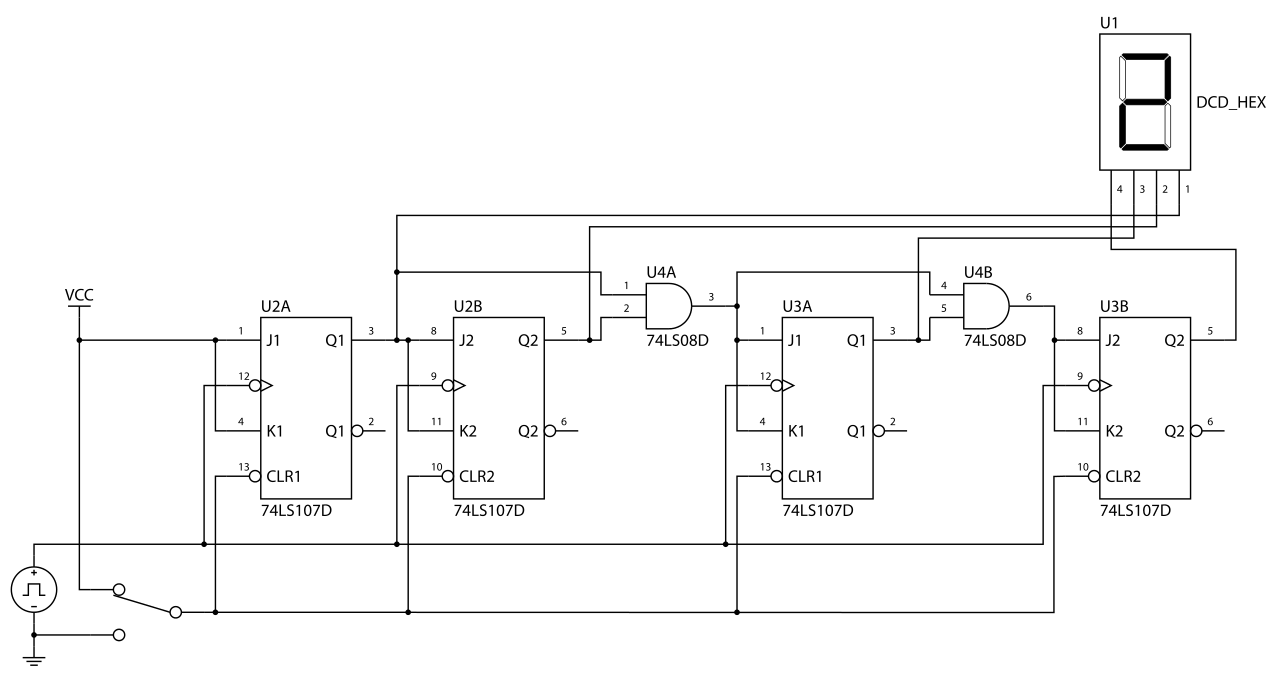
\includegraphics[width=\textwidth]{figs/schematic.png}
  \caption{Schematic}
  \label{fig:sche}
\end{figure}


\end{document}
% do not put anything after this

